\documentclass[11pt,          % font size: 11pt or 12pt
               phd,           % degree:    ms or phd
               doublespacing % spacing: onehalfspacing or doublespacing
               ]{ncsuthesis}

%%----------------------------------------------------------------------------%%
%%------------------------------ Import Packages -----------------------------%%
%%----------------------------------------------------------------------------%%

\usepackage{booktabs}  % professionally typeset tables
\usepackage{amsmath}%,amssymb,amsfonts}
\usepackage{textcomp}  % better copyright sign, among other things
%\usepackage{xcolor}
\usepackage{lipsum}    % filler text
% LEE \usepackage{subfig}    % composite figures
\usepackage{outlines} % for bullets

\usepackage[%
    font={small,sf},
    labelfont=bf,
    format=hang,    
    format=plain,
    margin=0pt,
    width=0.8\textwidth,
]{caption}
\usepackage[list=true]{subcaption}

\usepackage{url}


\usepackage{geometry} 
\usepackage{units}
\usepackage[binary-units=true]{siunitx}
\usepackage{pst-plot}
\usepackage{pgfplots}

% for quotes
\usepackage[utf8]{inputenc}
\usepackage{quotchap}
\usepackage{epigraph}
\usepackage{quotchap}
\usepackage{csquotes}

% help reduce whitespace
%\usepackage{savetrees}
%%ORTIZ PACKAGES


%%%%%%%%%%%%%%%%%%%%%%%%%%%%%%%%%%%%%%%%%%
%%%%%%%%%%% Old bibliography commands
%%%%%%%%%%%%%%%%%%%%%%%%%%%%%%%%%%%%%%%%%%5
%\usepackage[super,sort&compress,comma,square,authoryear]{natbib} %\cite command %Added by Ortiz

%use the following line with plainnat
%\usepackage[super,sort&compress,comma,square,numbers]{natbib} %\cite command %Added by Ortiz
%\usepackage{natbib}

%\usepackage[style=alphabetic,natbib=true,backend=bibtex
%sorting=nyt,firstinits=true,isbn=false,doi=false,url=false]{biblatex} %couldn't get backend=biber to work

%\usepackage{filecontents}

%\bibliography{Ortiz-thesis2}
%\bibliographystyle{plain}


%%%%%%%%%%%%%%%%%%%%%%%%%%%%%%%%%%%%%%%%%%
%%%%%%%%%%% Hack for alphanumeric bibliography
%%%%%%%%%%%%%%%%%%%%%%%%%%%%%%%%%%%%%%%%%%5
\RequirePackage[
			style=alphabetic,%numeric-comp,%authoryear-comp,%
			sorting=nyt,%ynt					
			hyperref=true, %	
			firstinits=true,%
			backend=bibtex,
			natbib=true,
			url=false,
			isbn=false,
			maxnames=2, %for et al to be used
			maxalphanames=1, %to avoid printing a + for every et al in the abbreviation
			doi=false]{biblatex}		
			

%needed to do et al after two names
%http://tex.stackexchange.com/questions/44048/use-et-al-in-biblatex-custom-style
\renewcommand*{\finalnamedelim}{\addspace\&\space}

%Simplify abbreviation (the default uses either one or two authors and it indicates et al with a +)
%The following five lines make it so that only the first author is used in the abbreviation
%http://tex.stackexchange.com/questions/27956/label-only-from-first-author
\renewcommand*{\labelalphaothers}{}
    \renewcommand*{\intitlepunct}{}
    \DefineBibliographyStrings{german}{in={}}
    \DefineBibliographyStrings{english}{in={}}
    \DeclareNameAlias{sortname}{last-first}
    \DeclareNameAlias{default}{last-first}
	
%\AtEveryCitekey{\ifciteseen{}{\defcounter{maxnames}{99}}} %authoryear			
\DeclareFieldFormat[article,periodical]{volume}{\mkbibbold{#1}}
\makeatletter

\newrobustcmd*{\parentexttrack}[1]{%
  \begingroup
  \blx@blxinit
  \blx@setsfcodes
  \blx@bibopenparen#1\blx@bibcloseparen
  \endgroup}

\AtEveryCite{%
  \let\parentext=\parentexttrack%
  \let\bibopenparen=\bibopenbracket%
  \let\bibcloseparen=\bibclosebracket}

\makeatother
\renewcommand{\cite}[1]{\parencite{#1}}


\renewbibmacro{in:}{%
  \ifentrytype{article}{}{%
  \printtext{\bibstring{in}\intitlepunct}}}
  
\AtEveryBibitem{\clearfield{month}}

\AtEveryBibitem{\clearfield{language}}
%%%%%%%%%%%%%%%%%%%%%%%%%%%%%%%%%%%%%%%%%%%%%

%\addbibresource{Ortiz-thesis2.bib}
%\addbibresource{Ortiz-thesisURL.bib}
\addbibresource{LeeBaker-thesis.bib}

 \defbibheading{myheading}[BIBLIOGRAPHY]{
 \chapter*{#1}
 %\centerline{\bf{#1}}
 \markboth{#1}{#1}}

%\usepackage{amsmath,amssymb,amsfonts} %amssymb and amsfonts cannot be used in conjunction with mdput
%\usepackage{graphicx,subfig}% Include figure files
\usepackage{dcolumn}% Align table columns on decimal point
\usepackage{bm}% bold math
%\usepackage{hyperref}% add hypertext capabilities
%\usepackage{hypernat}% make hyperref and natbib work together
\usepackage{cancel}
\usepackage{verbatim}% multiline commenting
\usepackage{ifthen}
\usepackage{url}
\usepackage{sectsty}
\usepackage{balance} 
%\usepackage{caption}
\usepackage{graphicx} %eps figures can be used instead
\usepackage{lastpage}
\usepackage[format=plain,justification=RaggedRight,singlelinecheck=false,font=small,labelfont=bf,labelsep=space]{caption} 
\usepackage{fancyhdr}
\pagestyle{fancy}

%http://tex.stackexchange.com/questions/100817/error-when-using-bc-from-abbrevs-in-caption
%Getting BC
\usepackage{abbrevs}
\usepackage{etoolbox}
\robustify{\DateMark} % after having loaded abbrevs

\usepackage{units} %Needed to solve bug from citation Hydrodynamics in 21/2 dimensions
%see http://www.latex-community.org/viewtopic.php?f=5&t=989

\usepackage[sharp]{easylist} %used for brainstorming purposes 
%\usepackage{mathabx} % used for \Asterisk for convolution %conflicts with \widering

%compile on single pass
%\usepackage[backend=biber,...]{biblatex}


%%%%%%%%%%%%
%%% Hack to make chapters start on odd pages
% http://tex.stackexchange.com/questions/73591/how-to-have-a-blank-even-page-before-every-chapter
%%%%%%%%%%%%
%\newcommand{\ensureoddstart}{\checkoddpage\ifoddpage\else\newpage\mbox{}\fi}
%\newcommand{\ensureoddstart}{}


%%%Fancy tables
%http://tex.stackexchange.com/questions/94032/fancy-tables-in-latex
% Lee \usepackage[table]{xcolor}
% Lee \usepackage{array,booktabs}
% Lee \usepackage{colortbl}
% Lee \newcolumntype{L}{@{}>{\kern\tabcolsep}l<{\kern\tabcolsep}}



%%%%%%%%%%
%%%%% Hack to allow more levels in outline
%%%%%%%%%%
%\setcounter{secnumdepth}{5}
%\setcounter{tocdepth}{5} %may violate ETD
%Usage http://pleasemakeanote.blogspot.com/2010/06/how-to-activate-subsubsubsection-in.html
%\section{} % level 1
%\subsection{} % level 2
%\subsubsection{} % level 3
%\paragraph{} % level 4 - equivalent to subsubsubsection
%\subparagraph{} % level 5

%http://tex.stackexchange.com/questions/60209/how-to-add-an-extra-level-of-sections-with-headings-below-subsubsection
\usepackage{titlesec}

\setcounter{secnumdepth}{4}

\titleformat{\paragraph}
{\normalfont\normalsize\bfseries}{\theparagraph}{1em}{}
\titlespacing*{\paragraph}
{0pt}{3.25ex plus 1ex minus .2ex}{1.5ex plus .2ex}

%%%%%%%%%%%%%%%%%%%%%%%%%%
%%%% Hack for containing figures within sections
%%%%%%%%%%%%%%%%%%%%%%%%%%%%
%http://ctan.org/pkg/placeins
\usepackage{placeins}
%De�fines a \FloatBar�rier com�mand, be�yond which floats may not pass; use�ful, for ex�am�ple, to en�sure all floats for a sec�tion ap�pear be�fore the next \sec�tion com�mand.

%%%Hack for centering all figures
%\makeatletter
%\g@addto@macro\@floatboxreset\centering
%\makeatother

%%----------------------------------------------------------------------------%%
%%---------------------------- Formatting Options ----------------------------%%
%%----------------------------------------------------------------------------%%
%%

%% -------------------------------------------------------------------------- %%
%% Disposition format -- any titles, headings, section titles
%%  These formatting commands affect all headings, titles, headings,
%%  so sizing commands should not be used here.
%%  Formatting options to consider are
%%     +  \sffamily - sans serif fonts.  Dispositions are often typeset in
%%                    sans serif, so this is a good option. 
%%     +  \rmfamily - serif fonts
%%     +  \bfseries - bold face
%\dispositionformat{\sffamily\bfseries}   % bold and sans serif
\dispositionformat{\bfseries}            % bold and serif

%% -------------------------------------------------------------------------- %%
%% Formatting for centered headings - Abstract, Dedication, etc. headings
%%  This is where one might put a sizing command.
%%  \MakeUppercase can be used to typeset all headings in uppercase.
\headingformat{\large\MakeUppercase}   % All letters uppercase
%\headingformat{\large}                % Not all uppercase
%\headingformat{\Large\scshape}        % Small Caps, used with serif fonts.

%% Typographers recommend using a normal inter-word space after
%% sentences. TeX's default is to add an wider space, but \frenchspacing
%% gives a normal spacing. Comment out the following line if you prefer
%% wider spaces between sentences.
\frenchspacing


%% -------------------------------------------------------------------------- %%
%%  Optional packages
%%    A number of compatible packages to improve the look and feel of
%%    your document are available in the file optional.tex 
%%    (For example, hyperlinks, fancy chapter headings, and fonts)
%% To use these options, uncomment the next line and see optional.tex
%%  Optional Packages to consider.   These packages are compatible with
%%    ncsuthesis.  

%% -------------------------------------------------------------------------- %%
%% Fancy chapter headings
%%  available options: Sonny, Lenny, Glenn, Conny, Rejne, Bjarne
%\usepackage[Sonny]{fncychap}
\usepackage[Rejne]{fncychap}

%%----------------------------------------------------------------------------%%
%% Hyperref package creates PDF metadata and hyperlinks in Table of Contents
%%  and citations.  Based on feedback from the NCSU thesis editor, 
%%  the links are not visually distinct from normal text (i.e. no change
%%  in color or extra boxes).
\usepackage[
  pdfauthor={Carlos Pompeyo Ortiz},
  pdftitle={Rigidity of Microsphere Heaps},
  pdfcreator={pdftex},
  pdfsubject={NC State ETD Thesis},
  pdfkeywords={microfluidics, hard sphere, jamming, suspension, rigidity, friction, microscopy},
  colorlinks=true,
  linkcolor=black,
  citecolor=black,
  filecolor=black,
  urlcolor=black,
]{hyperref}


%% -------------------------------------------------------------------------- %%
%% Microtype - If you use pdfTeX to compile your thesis, you can use
%%              the microtype package to access advanced typographic
%%              features.  By default, using the microtype package enables
%%              character protrusion (placing glyphs a hair past the right 
%%              margin to make a visually straighter edge)
%%              and font expansion (adjusting font width slightly to get 
%%              more favorable justification).
%%              Using microtype should decrease the number of lines
%%              ending in hyphens.
\usepackage{microtype}


%%----------------------------------------------------------------------------%%
%% Fonts 

%% ETD guidelines don't specify the font.  You can enable the fonts
%%  by uncommenting the appropriate lines.  Using the default Computer 
%%  Modern fonts is *not* required.  A few common choices are below.
%%  See http://www.tug.dk/FontCatalogue/ for more options.

%% Serif Fonts -------------------------------------------------
%%  The four serif fonts listed here (Utopia, Palatino, Kerkis,
%%  and Times) all have math support.


%% Utopia
\usepackage[T1]{fontenc}
\usepackage[adobe-utopia]{mathdesign}

%% Palatino
%\usepackage[T1]{fontenc}
%\usepackage[sc]{mathpazo}
%\linespread{1.05}

%% Kerkis
%\usepackage[T1]{fontenc}
%\usepackage{kmath,kerkis}

%% Times
%\usepackage[T1]{fontenc}
%\usepackage{mathptmx}


%% Sans serif fonts -------------------------

%\usepackage[scaled]{helvet}  % Helvetica
%\usepackage[scaled]{berasans} % Bera Sans

%solve bug from fancyhdr in optional
%http://nw360.blogspot.com/2006/11/latex-headheight-is-too-small.html
\setlength{\headheight}{14pt}

%%----------------------------------------------------------------------------%%
%%---------------------------- Content Options -------------------------------%%
%%----------------------------------------------------------------------------%%
%% Size of committee: 3, 4, 5, or 6 -- this number includes the chair
\committeesize{4}

%% Members of committee
%%  Each of the following member commands takes an optional argument
%%   to specify their role on the committee.
%%  For co-chairs, use the commands:
%%      \cochairI{Doug Dodd}
%%      \cochairII{Chris Cox}
%%
\chair{Paul Franzon}
\memberI{Winser Alexander}
\memberII{Gregory Byrd}
\memberIII{Richard Warr}   % unnecessary if committeesize=3


%% Student writing thesis, \student{First Middle}{Last}
\student{Lee B.}{Baker} % a full middle name
%\student{John Mark}{Smith} % a full middle name
%\student{John M.}{Smith} % a middle initial

%% Degree program
\program{Electrical Engineering}

%% Thesis Title
%%  Keep in mind, according to ETD guidelines:
%%    +  Capitalize first letter of important words.
%%    +  Use inverted pyramid shape if title spans more than one line.
%%
%%  Note: To break the title onto multiple lines, use \break instead of \\.
%\thesistitle{A North Carolina State University Sample \LaTeX{} Thesis \break 
%with a Title So Long it Needs a Line Break}
\thesistitle{Design of a 3DIC system to aid in the acceleration of systems that \break employ multiple instances of artificial neural networks}

%% Degree year.  Necessary if your degree year doesn't equal the current year.
%\degreeyear{1995}


%%----------------------------------------------------------------------------%%
%%---------------------------- Personal Macros -------------------------------%%
%%----------------------------------------------------------------------------%%

%% A central location to add your favorite macros.

%% A few examples to get you started.
\newcommand{\uv}[1]{\ensuremath{\mathbf{\hat{#1}}}}
\newcommand{\bo}{\ensuremath{\mathbf{\Omega}}}
\newcommand{\eref}[1]{Eq.~\ref{#1}}
\newcommand{\fref}[1]{Fig.~\ref{#1}}
\newcommand{\tref}[1]{Table~\ref{#1}}
\newcommand{\del}{\nabla}
\renewcommand{\exp}[1]{e^{#1}}
\newcommand{\Conv}{\mathop{\scalebox{1.5}{\raisebox{-0.2ex}{$\ast$}}}}%


\usepackage{color}
%\newcommand{\NEW}[1]{\textcolor{blue}{#1}}
\newcommand{\NEW}[1]{#1}
\newcommand{\COMMENT}[1]{\textcolor{green}{#1}}


\newcommand{\NOTER}[1]{\textcolor{orange}{#1}}
\newcommand{\NOTEC}[1]{\textcolor{blue}{#1}}
\newcommand{\NOTEK}[1]{\textcolor{magenta}{#1}}

\newcommand{\mum}{\ensuremath{{\mu}\text{m}}}

%This makes it so that you can add short paths in your .tex by including the folders where you store your images in the search path
\graphicspath{{./Chapter-1/figs/}{./Chapter-2/figs/}{./Chapter-3/figs/}{./Chapter-4/figs/}{./Chapter-5/figs/}{./Chapter-6/figs/}}


%%----------------------------------------------------------------------------%%
%%---------------------------- Plotting --------------------------------------%%
%%----------------------------------------------------------------------------%%
%% Added Lee

% axis style
\pgfplotsset{every axis/.append style={
                    axis x line=middle,    % put the x axis in the middle
                    axis y line=middle,    % put the y axis in the middle
                    axis line style={<->}, % arrows on the axis
                    xlabel={$x$},          % default put x on x-axis
                    ylabel={$y$},          % default put y on y-axis
                    }}
% grid style
\pgfplotsset{
  grid style = {
    dash pattern = on 0.05mm off 1mm,
    line cap = round,
    black,
    line width = 0.5pt
  }
}
% line style
\pgfplotsset{myBlueStyle/.style={color=blue,no marks,line width=1pt,-}} 
\pgfplotsset{myBlackStyle/.style={color=blue,no marks,line width=1pt,-}} 
\pgfplotsset{myBlueThickStyle/.style={color=blue,no marks,line width=2pt,-}} 
\pgfplotsset{myBlackThickStyle/.style={color=black,no marks,line width=2pt,-}} 

% arrow style: stealth stands for 'stealth fighter' 
\tikzset{>=stealth}

%\DeclarePairedDelimiter\ceil{\lceil}{\rceil}
%\DeclarePairedDelimiter\floor{\lfloor}{\rfloor}

%%---------------------------------------------------------------------------%%
\usepackage{calc}
%% Capital letter height
\newlength{\chaptercapitalheight}
\settoheight{\chaptercapitalheight}{D}
\newlength{\chapterfootskip}
\setlength{\chapterfootskip}{\chaptercapitalheight}
\addtolength{\chapterfootskip}{2\baselineskip}
\addtolength{\chapterfootskip}{0.5ex}  % A little extra space to ensure there are 2 full double spaced lines
%\def\chapterfootskipnum{\chapterfootskip}
\renewcommand{\listfigurename}{LIST OF FIGURES}
\renewcommand{\listtablename}{LIST OF TABLES}
\renewcommand{\bibname}{BIBLIOGRAPHY}

%\renewcommand{\cfttoctitlefont}{\centering\ncsu@headingformat}


%http://tex.stackexchange.com/questions/47184/height-of-figure-caption-textheight
\newlength\graphht
\newcommand\calculategraphicstargetheight[1]{%
     \setlength\graphht{\textheight 
                       -\parskip
                       -\abovecaptionskip -\belowcaptionskip
                       -(12pt * #1) % assuming baselineskip of 12pt in caption
                       -\chapterfootskip
                       }}

%\usepackage{titlesec}

%landscape support in fancyhdr from http://tex.stackexchange.com/questions/9071/how-to-translate-and-rotate-the-heading-of-landscaped-pages
\usepackage{pdflscape}
\usepackage{tikz}
\fancypagestyle{lscapedplain}{%
  \fancyhf{}
  \fancyfoot{%
    \tikz[remember picture,overlay]
      \node[outer sep=1cm,above,rotate=90] at (current page.east) {\thepage};}
\renewcommand{\headrulewidth}{0pt} 
\renewcommand{\footrulewidth}{0pt}
}

                      
\begin{document}
\pagestyle{plain}
%%---------------------------------------------------------------------------%%
\frontmatter

%% ------------------------------ Abstract ---------------------------------- %%
\begin{abstract}

%\lipsum[1-6]

Although Artificial Neural Networks (ANN) have been known about for many decades, it hasnt been until the last few years that
they have demonstrated efficacy in applications such as image recognition and voice recognition.
These ANNs have demonstrated significant improvements over what was considered to be state-of-the-art algorithms.

In most cases, ANNs must be "trained" to perform their function and these recent breakthoughs can, in a large part 
be attributed to the availability of "big" training data.

This data takes the form of images, recordings etc. and this along with the available storage capacity means that the required training data is now available 
to train these ANNs.

Artificial Neurons (AN) take their inspiration from neuron behavior observed in the mammalian brain, although
implementations are simplifications of what actually exists in the brain.
These simplifications range from attempts to emulate the actual spiking behavior of real neurons to ANs that simply encode the spiking behavior in the
form of a number or rate.

Surprisingly, the ANNs that have demonstrated the most efficacy are those that employ the more simpler rate-based ANs.
Now this may be in large part because these simpler rate-based ANs are easier to process or because large NNs employing the more complex spiking ANs have yet to
demonsrate improved efficacy in the various applications.
There is a belief that the more complex spiking neurons have the ability to outperform the simpler rate-based neurons but this work focuses on
the proven efficacy of ANNs formed from rate-based ANs.

The ANNs that have demonstrated to be most effective are a family of neural networks that can be described as Deep Neural Networks.
These DNNs are created by cascading layers of ANs to form a large, layered ANN. 
These ANNs are in most cases generate outputs in the form of a classification, such as the probability of an image containing a certain object
or the output of some approximated function, which might be the expected cost from making a stock trade.

Now researchers have experimented with various sized NNs for various applcations, but those that have demonstrated the most efficacy employ tens of thousands
of ANs.

In many implementations of these useful sized NNs, the performance is impacted by the memory bandwidth of the system. 
Much of the NN application specific (ASIC/ASIP) research has focused on taking advantage of the performance and ease of use of Static Random Access Memory or SRAM. 
These implementations can be shown to be effective with specific NN architectures, such as Convolutional NNs but in reality, these implementations do not provide the flexibility, 
storage capacity and deterministic performance required to implement all useful sized NNs.

In addition, it is this works belief that that real-world applications will employ multiple instances of these useful sized ANNs and current implementations will not
meet the demands of these multi NN systems.

\iffalse
Researchers have attempted to solve this with
the use of fast local SRAM. These implementations rely on the ANN being able to store data in the local SRAM and reuse that data without having to
constantly go to the main memory, which is often implemented in slower DRAM.
However, many DNNs do not exhibit this ability to reuse the contents of local SRAM, or not to the extent that makes these implementations acceptable.
Some work has included combining SRAM with DRAM but these implementations still exhibit poor performance with a wider family of ANNs.
\fi

One area of integrated circuit technology that hasnt been widely used in ANNs is 3-D integrated circuits (3DIC).  3DIC has the potential to increase connectivity, and thus bandwidth 
and keep power dissipation to within acceptable levels.

This work combines ANNs with 3DIC technology to demonstrate how a 3DIC dynamic random access memory (DRAM) memory can be combined with customized IC layers to produce a system providing
an acceptable level of performance in systems with multiple instances of various types of DNNs.

This work includes utilizing a customized 3D DRAM along with a system which includes a management layer which coordinates and executes ANN operations in the form
of unique instructions and a processing layer able to process data from the DRAM, via the manager at a bandwidth that meets the demands of a system employing
multiple ANNs.



\end{abstract}


%% ---------------------------- Copyright page ------------------------------ %%
%% Comment the next line if you don't want the copyright page included.
\makecopyrightpage

%% -------------------------------- Title page ------------------------------ %%
\maketitlepage

%% -------------------------------- Dedication ------------------------------ %%
\begin{dedication}
 \centering To my wife Mandy, my children Adam, Rachel and Paul and my parents Joan and Barry.
\end{dedication}

%% -------------------------------- Biography ------------------------------- %%
\begin{biography}
The author was born in a the United Kingdom to a working class family.  After performing poorly in high school he took a job in a local electronic engineering firm
under a vocational program.
After seeing the white coated "engineers" being called down from upstairs to solve the "big" problems, he decided he wanted to wear one
of those white coats (his dress sense was wanting).
The journey took him to Brighton Polytechnic, now Brighton University and a First Class Honours Degree in Electrical Engineering.
After working in the UK for a couple of years, he moved to the United States.
The journey included a family with a daughter and two son's.
The education continued with a Masters in Engineering from Villanova University and a Masters in Business Administration from North
Carolina State University.

With the family now being somewhat independent, he decided to make a career change which would hopefully include teaching.

That career change included enrolling in the Electrical Engineering PhD program at North
Carolina State University. This stage of the education journey has resulted in this dissertation.

%\begin{chapquote}{Lewis Carroll, \textit{Alice in Wonderland}}
%``Begin at the beginning,'' the King said, gravely, ``and go on till you
%come to an end; then stop.''
%\end{chapquote}
%\setlength{\epigraphwidth}{6in} 
%\epigraphfontsize{\small\itshape}
%\epigraph{do not stand still and do not let your past dictate your future}{--- \textup{Unknown}}
%\epigraph{do not stand }{--- \textup{Unknown}}

%\begin{savequote}[100mm]
%---When shall we three meet again
%in thunder, lightning, or in rain?
%---When the hurlyburly’s done,
%when the battle’s lost and won.
%\qauthor{Shakespeare, Macbeth}
%Cookies! Give me some cookies!
%\qauthor{Cookie Monster}
%\end{savequote}
%\begin{displayquote}

%\end{displayquote}
%\textcquote{do not stand still.}
%\textcquote{do not let your past dictate your future.}
%\blockquote{unknown}{do not let your past dictate your future.}
%\hyphenquote{american}{quote snippet in a different language}

And remember:

"do not stand still." and
"do not let your past dictate your future."

%"`foo"'

\end{biography}

%% ----------------------------- Acknowledgements --------------------------- %%
\begin{acknowledgements}
At a personal level, I would like to thank my wife Mandy and my children Adam, Rachel and Paul for their encouragement.

I would like to thank my advisor, Paul Franzon for his help in making this possible.

I would also like to thank my fellow students, especially Jong Beom, Josh, Sumon and Weifu for their healthy discussions and referring to me as Lee and not Sir or Mr. Baker.

\end{acknowledgements}


%% Lee
% Uncomment for dissertation (change to iftrue)
%\iffalse
\iftrue

\thesistableofcontents

\thesislistoftables

\thesislistoffigures

\fi


%%---------------------------------------------------------------------------%%
\mainmatter



\pagestyle{plain}
\newgeometry{margin=1in,lmargin=1.25in,footskip=\chapterfootskip, includehead, includefoot}
%\setcounter{chapter}{1}
%% Lee
%% In dissertation, change 
%    section* to chapter 
%    subsection* to section
%    subsubsection* to subsection

\chapter{Introduction}
%\section{Introduction}
\label{sec:chap-one}

Recently, there has been much interest in the use of artificial neural networks in systems that employ tasks such as image recognition\cite{krizhevsky2012imagenet}, text recognition\cite{qiu2013parallel} and game playing\cite{maddison2014move}.
In particular, in the field of image recognition these artificial neural network models have demonstrated superior performance
over other state-of-the-art technology\cite{krizhevsky2012imagenet}.
%There is reason to believe 
These artificial neural networks will continue to be applied to numerous other areas such as voice recognition, text recognition, 
face recognition and autonomous control.

Artificial neural networks (ANN) take their inspiration from neuron behavior observed in the mammalian brain, although implementations are simplifications of what actually exists in the brain.

The mammalian neuron is a cell that receives input and generates output in the form of electrical and chemical processes.
The neuron has a cell body (or soma), a group of dendrites which provide the inputs from other cells, a cell body, an axom which generates the output signals, and the axom terminals which are the outputs of the cell.
The connection from a cells output, or axom terminal to another cells input, or dendrite is known as a synapse. 
The connection in the synapse is a chemical process stimulated by electrical impulses.
The neuron can be seen in figure \ref{fig:neuron}.

The connection from one cell to another has both an associated delay and a strength. The strength of the connection can be influenced by the size of the pre-synaptic neuron spike or by the pre-synaptic neuron generating a series of spikes rather than a single spike.

\begin{figure}[!t]
% the [] contains position info e.g. [!t] means here
\centering
\captionsetup{justification=centering}
\captionsetup{width=.9\linewidth}
\centerline{
\mbox{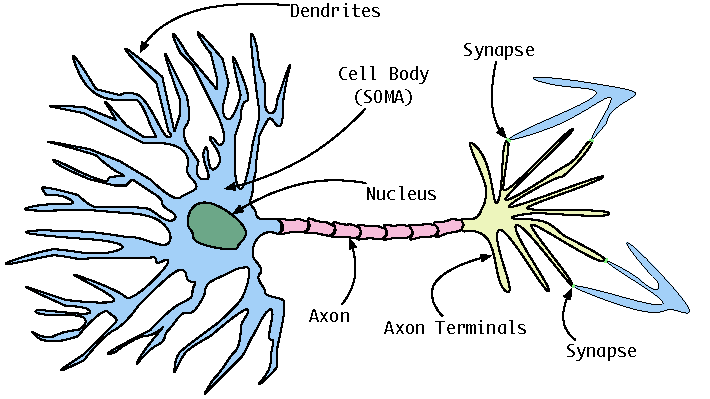
\includegraphics[width=4.0in]{Neuron.pdf}}
}
\caption{Neuron}
\label{fig:neuron}
\end{figure}



\iftrue
So it is known that mammalian neurons generate "spikes" in response to inputs which for humans include sight, touch, sound etc.. This spiking behavior is often referred to as the neuron being activated.
When these neurons are activated, their spikes propagate to other neurons. Under certain conditions, the combination of the various inputs to a neuron cause it to activate. 
A particular neuron may have many hundreds, perhaps thousands of other neurons connected to its "input".
These input neurons are referred to as pre-synaptic neurons. These pre-synaptic neurons may provide input to many neurons which are referred to as post-synaptic neurons.
A particular neuron can get activated by a particular arrival pattern of pre-synaptic neuron spikes or simply by the intensity of the pre-synaptic spikes. 

The spiking behavior of a neuron also varies and many spiking patterns have been observed. 
It is the delays and strength of the connections that contain the "information" in the neural network.
In simple terms, if a neuron is activated by its pre-synaptic neurons, then the activation of the neuron means a pattern has been detected which will influence a reaction.
In mammalian terms, that might be the detection of a threat from both smell and sight neurons and the reaction is to control muscles resulting in flight.

The various chemical and electrical processes that result in the generation and propagation of these neuron spikes is beyond the scope of this dissertation, but how neurons and networks of neurons are artificially emulated is what we will duscuss next.


\subsection*{Artificial Neural Networks}
\label{sec:Artificial Neural Networks}

When modeling these neurons in artificial neural networks, the outputs of the neuron models either generate actual spikes or
produce a value which is proportional to the rate at which spikes occur.
These artificial neural networks can be categorized as rate-based coded or spike time coded neurons.

When used in networks of neurons, both model types employ a connection weight between the pre and post-synaptic neuron, however, the
spiking neuron network also introduces a time delay associated with the connection.
Although the spiking neural network more closely models the behavior of real neurons, over the last 20 years there 
have been breakthroughs in the configuring of rate-based models especially in the application of the back-propagation
algorithm and stochastic gradient descent. Along with the abundance of data now available in the form of voice, images etc. to "teach" these networks
using back-propagation, most of the effective applications of artificial neural networks have employed these rate-based models.
Our research will focus on these rate-based models which we will now refer to as ANNs.
\fi

To approach the capabilities observed in human behavior, such as object recognition these ANNs become very large.
They often utilize hundreds of thousands of neurons to implement what we would consider a relatively straightforward task.
For example, a "useful" ANN similar to that described in \cite{krizhevsky2012imagenet} that is used
to recognize up to 1000 different object classes has a network size of approximately 650,000 neurons and 
630 million synaptic connections \cite{krizhevsky2012imagenetPreso}. 
Many applications require multiple instances of ANNs of similar size to the ANN described in \cite{krizhevsky2012imagenet}.
For example employing multiple cameras in a drone or automobile each with an image recognition ANN\cite{krizhevsky2012imagenet}\cite{bojarski2016end}.
These implementations have very large memory and processing requirements.
The requirements of these applications are typically satisified by employing multiple graphics processor units(GPU).
These multiple GPU systems have high real-estate and power requirements that may exceed the target applications requirements.

This research explores a 3DIC solution using a custom organized 3DIC memory in conjunction with unique data structures and custom processing modules to significantly reduce the 
area and power footprint of an application that needs to support the processing associated with multiple ANNs.


Artificial Neural Networks are a network of inter-connected processing elements inspired by the 
connectivity and processing observed in the brain.
% Uncomment for dissertation

They are characterized by the connections between a pre-synaptic neuron and a post-synaptic
neuron having a weight which determines the impact the pre-synaptic neuron has on the 
"activation" of a post-synaptic neuron.
Typically the processing portion of the neuron performs a multiplication and accumulation on the outputs from all
the pre-synaptic neurons followed by a non-linear "activation" function, such as a rectified linear unit or sigmoid function to create the neuron output.

It is well understood a single layer of these neurons can be configured to perform a linear function approximation.
A collection of these neurons, when connected in layers with one layers neurons connected to
the next layers neurons, are known to be able to act as non-linear function approximators.
As well as being effective function approximators, these neurons can be configured to act as 
classifiers, attractor networks or associative memories.
A simple example of an ANN can be seen in \fref{fig:simpleNetwork} and the contents of an artificial neuron 
with the multiplication and summation stages and the activation function $f(x)$ can be seen in \fref{fig:cellContents}. 


\begin{figure}
\centering
\begin{subfigure}{.65\textwidth}
  \centering
  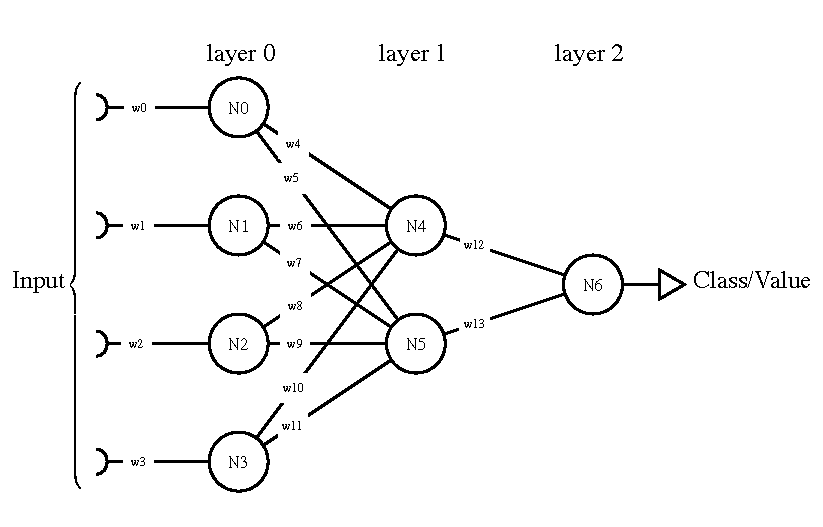
\includegraphics[width=0.9\textwidth]{Chapter-1/figs/simpleANN}
  \captionsetup{justification=centering, skip=-20pt}
  \caption{network}
  \label{fig:simpleNetwork}
\end{subfigure}%
\begin{subfigure}{.3\textwidth}
  \centering
  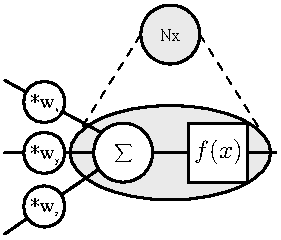
\includegraphics[width=0.7\textwidth]{Chapter-1/figs/cellContents}
  \captionsetup{justification=centering, skip=3pt}
  \caption{neuron}
  \label{fig:cellContents}
\end{subfigure}
\captionsetup{justification=centering, skip=10pt}
\caption{Simple Artificial Neural Network}
\label{fig:Simple Artificial Neural Network}
\end{figure}

For the most part, different ANNs are characterized by the function contained in the
processing element, how the neurons are interconnected and how the weights of the inter-connections are configured or learnt.
Most of the effective applications of ANNs require 10's of thousands of neurons and millions of synaptic connections.
When the entire network must generate a result in near real-time, the result is a system requiring billions
of floating point operations per second. When multiple ANNs need to be processed in parallel, the power and area requirements may not always be satisifed
using current technology.

%%
%%When multiple of these networks must be processed in parallel \cite{qiu2013parallel}\cite{bojarski2016end},
%%we quickly exceed the capabilities of current state-of-the-art technology.
%-------------------------------------------------------------------------------------
% FIXME - do we need activation function figures?
% start FIXME
\iftrue
Some typical examples of the 
activation function can be seen in \fref{fig:Typical neuron activation functions}.

\begin{figure}
\centering
\begin{subfigure}{.32\textwidth}
  \centering
    \begin{tikzpicture}[scale=0.55]
      \begin{axis}[
          xlabel={$$},
          ylabel={$$},
          xlabel style={below right},
          ylabel style={above left},
          title={Sigmoid},
          %grid = major,
          xmin=-6,xmax=6,
          ymin=0,ymax=1,
          legend style={draw=none, fill=white},      
          legend pos= outer north east
          ]
          \addplot[myBlackThickStyle] expression[domain=-6:6,samples=100]{1/(1+e^(-x))} 
                      node at (axis cs:3,0.7){}; 
          %\legend{{\large $f(x)=\frac{1}{1+e^{-t}}$}}
      \end{axis}
    \end{tikzpicture}
  \captionsetup{justification=centering, skip=3pt}
  \caption{Sigmoid}
  \label{fig:SigmoidFunction}
\end{subfigure}%
\begin{subfigure}{.32\textwidth}
  \centering
    \begin{tikzpicture}[scale=0.55, transform shape]
      \begin{axis}[
          xlabel={$$},
          ylabel={$$},
          xlabel style={below right},
          ylabel style={above left},
          title={ReLu},
          xmin=-1,xmax=1,
          ymin=0,ymax=1,
          legend style={draw=none, fill=white},      
          legend pos= outer north east
          ]
           \addplot[myBlackThickStyle] expression[domain=0:1,samples=100]{x} node at (axis cs:0.6,0.15){}; 
           \addplot[myBlackThickStyle] expression[domain=-1:0,samples=100]{0};       
           %\legend  {{ $f(x)= \begin{cases} 0,      &\text{if $x < 0$;}\\   x,       &\text{otherwise.}  \end{cases}$}}  
      \end{axis}
    \end{tikzpicture}
  \captionsetup{justification=centering, skip=3pt}
  \caption{ReLu}
  \label{fig:ReLuFunction}
\end{subfigure}
\begin{subfigure}{.32\textwidth}
  \centering
    \begin{tikzpicture}[scale=0.55]
      \begin{axis}[
          xlabel={$$},
          ylabel={$$},
          xlabel style={below right},
          ylabel style={above left},
          title={Saturation},
          xmin=-2,xmax=2,
          ymin=-1.5,ymax=1.5,
          legend style={draw=none, fill=white},      
          legend pos= outer north east
          ]
           \addplot[myBlackThickStyle] expression[domain=-1:1,samples=100]{x} node at (axis cs:0.6,0.15){}; 
           \addplot[myBlackThickStyle] expression[domain=-2:-1,samples=100]{-1};       
           \addplot[myBlackThickStyle] expression[domain=1:2,samples=100]{1};       
           %\legend  {{ $f(x)= \begin{cases} 1,      &\text{if $x \ge 1$;}\\ x,      &\text{if $-1<x<1$;}\\  -1,      &\text{if $x \le -1$;} \end{cases}$}}  
      \end{axis}
    \end{tikzpicture}
  \captionsetup{justification=centering, skip=3pt}
  \caption{Saturation}
  \label{fig:SaturationFunction}
\end{subfigure}
\captionsetup{justification=centering, skip=3pt}
\caption{Typical neuron activation functions}
\label{fig:Typical neuron activation functions}
\end{figure}

\fi
% end FIXME
%-------------------------------------------------------------------------------------

%%This research will target a family of ANNs that have demonstrated efficacy in
%%a family of popular applications. These applications have large neural networks requiring a large amount of memory 
%%to support weight storage and the requirement of processing multiple ANNs at or near real-time.
% FIXME - should I use this line or a version of it
%As mentioned in section \ref{sec:chap-one}, it is our belief that most useful applications of ANNs fall into this category.

%% Moved to chapter 3
%%\subsection*{Targeted Applications}
%%\label{sec:Targeted Applications}
%%
%%This work will target:
%%\begin{outline}
%%\renewcommand{\outlinei}{enumerate}
%%  \vspace{-3mm}
%%  \1 Brain-state-in-a-Box (BsB) and Cogent Confabulation (CC) because of their demonstrated efficacy in text recognition \cite{qiu2013parallel}.
%%    \vspace{-3mm}
%%    \2 The system described in \cite{qiu2013parallel} utilized 78 clusters with each cluster incorporating 22 Sony PS3 game stations and two NVidia GPU
%%       cards. The text recognition system was segmented into character recognition performed by the BsB networks and the word and sentence construction was
%%       performed by Cogent Confabulation.
%%       There is opportunity to accelerate BsB and potential to accelerate portions of the Cogent Confabulation networks.
%%  \vspace{-08mm}
%%  \1 Deep neural networks \cite{krizhevsky2012imagenet} because of their demonstrated efficacy in image recognition 
%%    \vspace{-3mm}
%%    \2 The application space includes autonomous navigation of automobiles \cite{bojarski2016end}
%%       with a need to process multiple deep neural networks simultaneously at real-time.
%%  \vspace{-3mm}
%%  \1 Reinforcement learning in the context of ANNs
%%    \vspace{-3mm}
%%    \2 The reinforcement learning algorithm employs deep neural networks in action-value function approximation \cite{mnih2013playing}. 
%%       Considering most environments will have very large state spaces,
%%       environment exploration will result in large numbers of action-value calculations and therefore acceleration will improve learning times.
%%       It should be noted that supporting reinforcement learning will require provisions for acceleration of back-propagation.
%%\end{outline}

%%---------------------------------------------------------------------------------------------------------
%%---------------------------------------------------------------------------------------------------------
%% FIXME
%% uncomment for dissertation
\iffalse

\subsubsection*{Brain-State-in-a-Box}

This ANN is an auto-associative memory implemented as a recursive neural network. The network employs the saturation function, shown in \fref{fig:SaturationFunction} 
as its activation function.
The network is trained to a set of attractor primitives as described in \cite{lillo1994synthesis}.
During inference, the network neurons are loaded with the state of the input which is typically a noisy version of one of the stored primitives.
The network is then iteratively processed until the value of each node approaches unity indicating the network has converged on a stored primitive.
The iterative process taking multiple passes through the neural network and that many BsB networks are employed in a given application
provides opportunity for a solution that provide acceleration and large storage.

\fi


\iffalse

\subsubsection*{Cogent Confabulation}

Cogent confabulation is a probabilistic model where the synaptic weight reflects the coexistence likelihood between symbols in different lexicons.
Each neuron represents a specific symbol in a lexicon and the activation value of each neuron is proportional to the co-existence likelihood between
the symbol the neuron represents and other symbols in the observation.

The weights are typically stored in the form of a matrix known as a knowledge base (KB).
What makes this ANN different is that the processing is not deterministic where with most neural networks, all neurons are processed in a regular fashion.
With cogent confabulation only neurons which have links to an observed or inferred symbol are processed.
An example of predicting a symbols likelihood from other observed symbols can be seen in \fref{fig:Cogent confabulation likelihood calculation}.
\begin{figure}[hbtp]
\centering
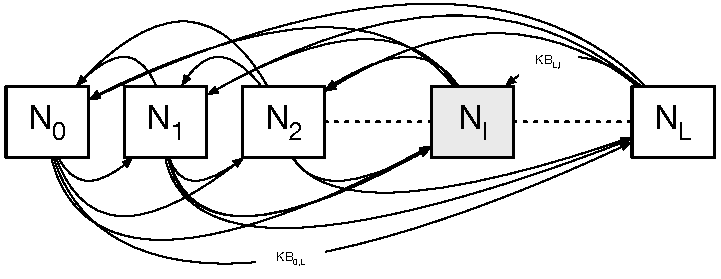
\includegraphics[width=0.4\textwidth]{Chapter-1/figs/CCnetwork}
\captionsetup{justification=centering, skip=3pt}
\caption{Cogent confabulation likelihood calculation}
\label{fig:Cogent confabulation likelihood calculation}
\end{figure}
There is no activation function employed with cogent confabulation neurons.

Cogent confabulation is often used in a process whereby a system converges on the most likely combination of symbols given an obervation \cite{qiu2013parallel}.
It is this converging and the raw size of the knowledge bases that provides opportunity for a solution that provides acceleration and large storage.

\fi


\iftrue

\subsubsection*{Deep Neural Networks}

A single layer of neurons is a linear classifier and therefore cannot be used to classify unless the classes can be separated using a linear function.
Even some simple cases cannot be linearly separated, an example often used is an exclusive-OR gate.
To allow classes in these cases to be linearly separated, the input space needs to be transformed.
Deep neural networks are ANNs that incorporate many layers of neurons which are often up to 10 layers deep.
These additional layers are incorporated to translate the space of the input so the various classes being identified can be separated using linear classifiers in the later
layers.
A very successful early example known as a convolutional neural network (CNN) is which in \cite{krizhevsky2012imagenet} was used to classify objects in images
and shown in \fref{fig:simple Imagenet network}.
\begin{figure}[hbtp]
\centering
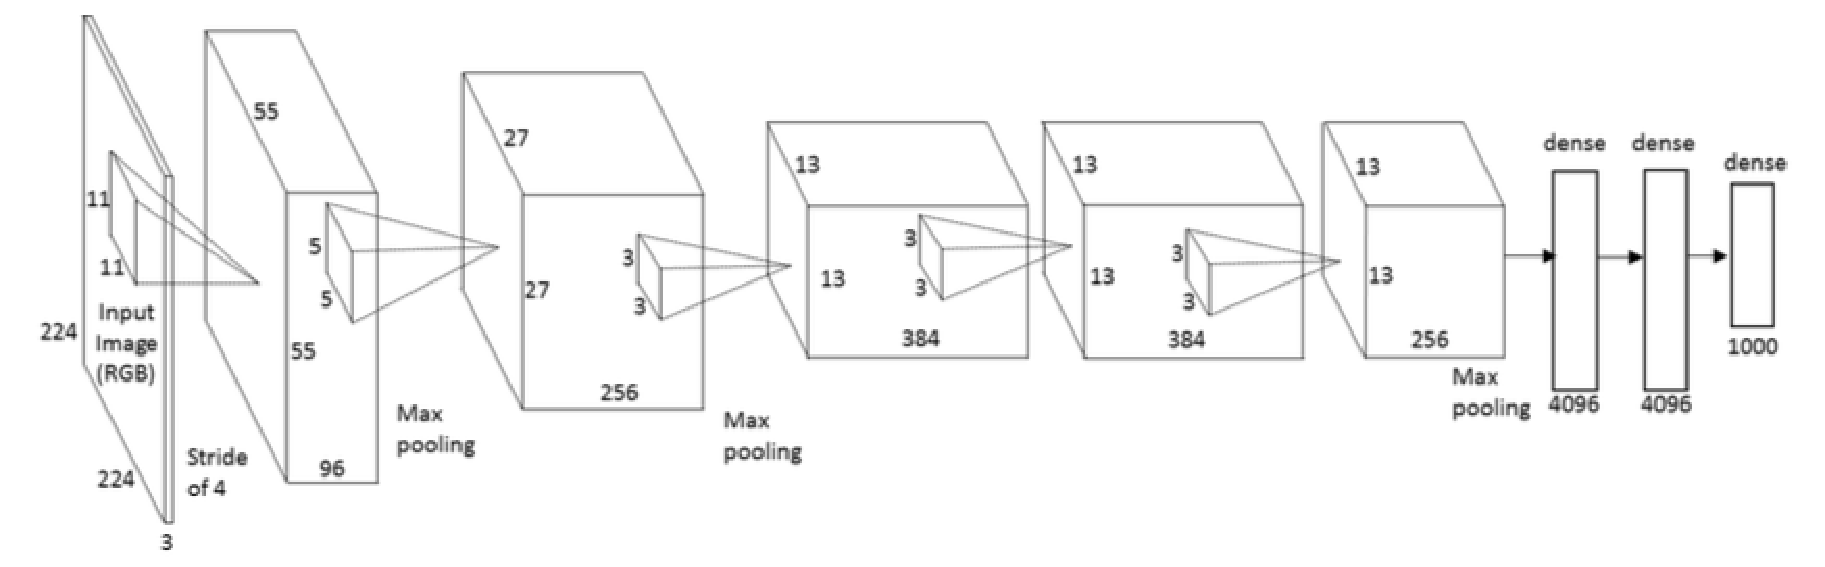
\includegraphics[width=0.9\textwidth]{Chapter-1/figs/deepNetworkShowingFeatureLayers}
\captionsetup{justification=centering, skip=-5pt}
\caption{Imagenet convolutional neural network from \cite{krizhevsky2012imagenetPreso}}
\label{fig:simple Imagenet network}
\end{figure}
These CNN's use the early layers to identify low-level features and later layers are used combine these features into yet more higher-level features.
Finally, the combination of high-level features are used to classify.
This layering is shown in \fref{fig:Deep network showing feature layers}.
\begin{figure}[hbtp]
\centering
\includegraphics[width=0.8\textwidth]{Chapter-1/figs/deepNetworkBlockDiagram}
\captionsetup{justification=centering, skip=5pt}
\caption{Deep network showing feature layers}
\label{fig:Deep network showing feature layers}
\end{figure}
Finally, a fully connected linear classify is used to classify the object using this translated input.
These deep neural networks can be used as classifiers or as function approximators as in our implementation of reinforcement learning.
In practice, useful deep neural networks are very large and often exceed the capacity of single GPU's. Therefore,  there is opportunity for a solution that provides
real-time acceleration and storage of of these systems.

\fi


\iftrue

\subsubsection*{Reinforcement Learning}
In the context of this work, reinforcement learning is the process by which a system identifies the actions to take to maximize reward.
For example, what actions should an aircraft take to avoid crashing (low reward) versus landing (high reward).
In this context of this work, we are discussing solving the action-reward function associated with a complex Markov-Decision-Process (MDP).
The action-reward function tells an agent operating in an environment the expected accumulated reward if an action is taken
in a particular state. The idea being the agent should always take the action that provides maximum expected reward.
The action-value function is defined for any state an agent may find itself in.
There are various dynamic programming methods employed to "learn" this action-value function and in most cases through repeated trials.
However, in most useful environments, the size of the state-space is too large to learn and/or store each states action-value table, therefore action-value function
approximators are used and deep neural networks are used as these approximators \cite{mnih2013playing}.
The focus of this work will be on accelerating the application of deep NNs to action-value function approximators.

\fi

%%---------------------------------------------------------------------------------------------------------
%%---------------------------------------------------------------------------------------------------------



%% Lee
%% In dissertation, change 
%    section* to chapter 
%    subsection* to section
%    subsubsection* to subsection

\chapter{Artificial Neural Networks}
%\section{Artificial Neural Networks}
\label{sec:chap-two}

Recently, there has been much interest in the use of artificial neural networks in systems that employ tasks such as image recognition\cite{krizhevsky2012imagenet}, text recognition\cite{qiu2013parallel} and game playing\cite{maddison2014move}.
In particular, in the field of image recognition these artificial neural network models have demonstrated superior performance
over other state-of-the-art technology\cite{krizhevsky2012imagenet}.
%There is reason to believe 
These artificial neural networks will continue to be applied to numerous other areas such as voice recognition, text recognition, 
face recognition and autonomous control.

Artificial neural networks (\ac{ann}) take their inspiration from neuron behavior observed in the mammalian brain, although implementations are simplifications of what actually exists in the brain.

The mammalian neuron is a cell that receives input and generates output in the form of electrical and chemical processes.
The neuron has a cell body (or soma), a group of dendrites which provide the inputs from other cells, a cell body, an axom which generates the output signals, and the axom terminals which are the outputs of the cell.
The connection from a cells output, or axom terminal to another cells input, or dendrite is known as a synapse. 
The connection in the synapse is a chemical process stimulated by electrical impulses.
The neuron can be seen in figure \ref{fig:neuron}.

The connection from one cell to another has both an associated delay and a strength. The strength of the connection can be influenced by the size of the pre-synaptic neuron spike or by the pre-synaptic neuron generating a series of spikes rather than a single spike.

\begin{figure}[!t]
% the [] contains position info e.g. [!t] means here
\centering
\captionsetup{justification=centering}
\captionsetup{width=.9\linewidth}
\centerline{
\mbox{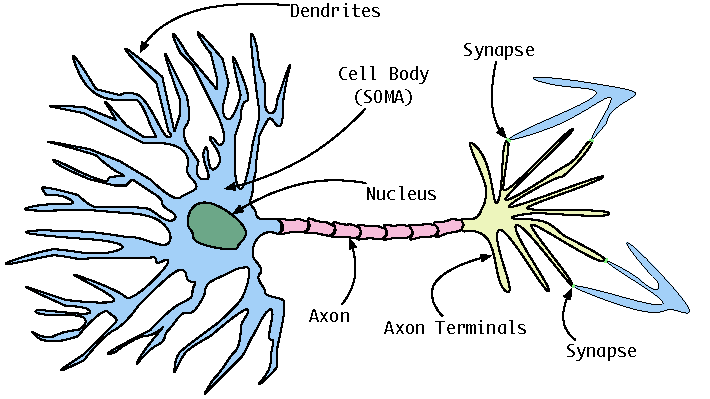
\includegraphics[width=4.0in]{Neuron.pdf}}
}
\caption{Artists impression of a Mammalian Neuron}
\label{fig:neuron}
\end{figure}



\iftrue
So it is known that mammalian neurons generate "spikes" in response to inputs which for humans include sight, touch, sound etc.. This spiking behavior is often referred to as the neuron being activated.
When these neurons are activated, their spikes propagate to other neurons. Under certain conditions, the combination of the various inputs to a neuron cause it to activate. 
A particular neuron may have many hundreds, perhaps thousands of other neurons connected to its "input".
These input neurons are referred to as pre-synaptic neurons. These pre-synaptic neurons may provide input to many neurons which are referred to as post-synaptic neurons.
A particular neuron can get activated by a particular arrival pattern of pre-synaptic neuron spikes or simply by the intensity of the pre-synaptic spikes. 

The spiking behavior of a neuron also varies and many spiking profiles have been observed, including single spikes, groups of spikes and repetitive spiking. 
It is believed that information is carried in the delay and strength of the connections and how pre-synaptic neurons combine to cause a neuron to activate.
In simple terms, if a neuron is activated by its pre-synaptic neurons, then the activation of the neuron means a pattern has been detected which will influence a reaction.
In mammalian terms, that might be the detection of a threat from both smell and sight neurons and the reaction is to control muscles resulting in flight.


The various chemical and electrical processes that result in the generation and propagation of these neuron spikes is beyond the scope of this dissertation, but how neurons and networks of neurons are artificially emulated is what we will discuss next.


%\section[NnSP]{NnSP{\cite{esmaeilzadeh2005nnsp}}}
\section[Artificial Neural Networks]{Artificial Neural Networks}
\label{sec:Artificial Neural Networks}

When modeling these neurons in artificial neural networks, the neuron models either generate actual spikes similar to actual neurons or
produce a value which is proportional to the rate at which spikes occur.
These artificial neural networks can be categorized as rate-based coded or spike time coded neurons.


When used in networks of neurons, both model types employ a connection weight between the pre and post-synaptic neuron, however, the spiking neuron network also introduces a time delay associated with the connection.

The spiking neuron model is characterized by:

\begin{outline}
  %\setlength{\baselineskip}{10pt}
  %\setlength{\itemsep}{12pt}
  %\setlength{\partopsep}{0pt}
  %\setlength{\parskip}{0pt}
  %\setlength{\parsep}{0pt}
  %\setlength{\topsep}{0pt}
  %\setlength{\itemindent}{\leftmargin}
  %\setlength{\leftmargin}{0pt}
        \1 Connections between neurons have both a strength and a delay
          \2 The pre-synaptic neuron output is multiplied by the connection weight and delayed
        \1 The weighted inputs from all pre-synaptic neurons are accumulated
        \1 The accumulated inputs drives an activation function
          \2 the activation function $f(x)$ is a spiking model is based on differential equations
          \2 many models have been proposed with varying levels of complexity
            \3 examples are:
              \4 Leaky integrate and fire
              \4 Izhikevich \cite{Iz2005} (see \fref{fig:Izhikevich Model})
         
\end{outline}

The Rate-based neuron model is characterized by:
\begin{outline}
        \1 Connections between neurons have only a strength
          \2 The pre-synaptic neuron output is multiplied by the connection weight
        \1 The weighted inputs from all pre-synaptic neurons are accumulated
        \1 The accumulated inputs drives an activation function
          \2 the activation function $f(x)$ is a non-linear function
          \2 early models used binary functions although in practice the function needs to be differentiable
            \3 examples are (see \fref{fig:Example Rated-Based Model Activation functions}):
              \4 sigmoid
              \4 rectified linear unit
\end{outline}

\begin{figure}
\centering
\begin{subfigure}{.4\textwidth}
  \centering
  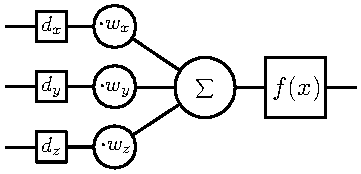
\includegraphics[width=0.85\textwidth]{SpikeBasedModel}
  \captionsetup{justification=centering, skip=5pt}
  \caption[Spiking Model]{Spiking Model}
  \label{fig:Spiking Model}
\end{subfigure}%
\begin{subfigure}{.4\textwidth}
  \centering
  \includegraphics[width=0.7\textwidth]{RatebasedModel}
  \captionsetup{justification=centering, skip=5pt}
  \caption{Rate-Based Model}
  \label{fig:Rate Based Model}
\end{subfigure}
\begin{subfigure}{.9\textwidth}
  \centering
  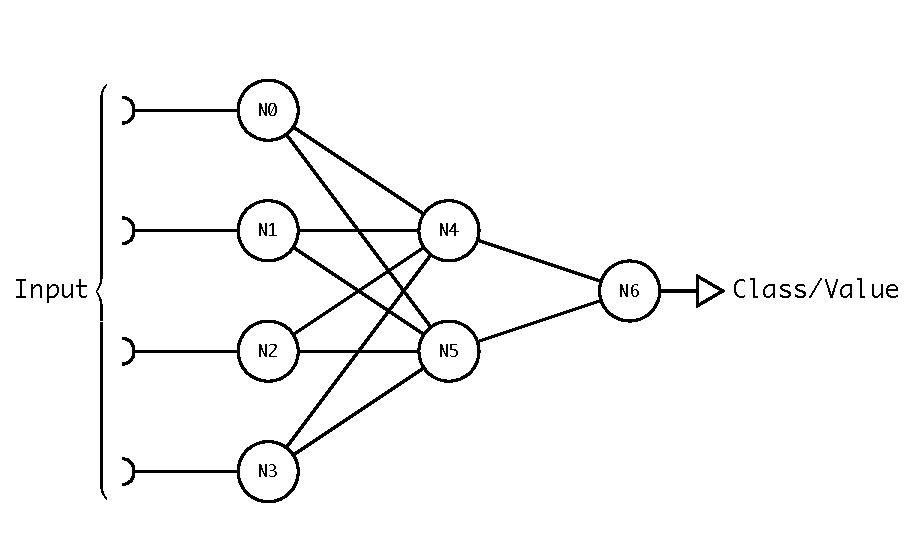
\includegraphics[width=0.7\textwidth]{SimpleNetwork}
  \captionsetup{justification=centering, skip=5pt}
  \caption{Network of Artificial Neurons}
  \label{fig:Network of ANs}
\end{subfigure}
\captionsetup{justification=centering, skip=6pt}
\caption[Artificial Neural Network]{Artificial Neurons and Network}
\label{fig:Artificial Neural Network}
\end{figure}

\begin{figure}
\centering
\begin{subfigure}{.3\textwidth}
  \begin{tikzpicture}[scale=0.5]
    \begin{axis}[
        title={Sigmoid},
        %grid = major,
        xmin=-6,xmax=6,
        ymin=0,ymax=1,
        legend style={draw=none, fill=white},      
        legend pos= outer north east
        ]
        \addplot[myBlueThickStyle] expression[domain=-6:6,samples=100]{1/(1+e^(-x))} 
                    node at (axis cs:3,0.7){}; 
        \legend{{\large $f(x)=\frac{1}{1+e^{-t}}$}}
    \end{axis}
  \end{tikzpicture}
  \captionsetup{justification=centering, skip=5pt}
  \caption{Sigmoid}
  \label{fig:Sigmoid}
\end{subfigure}%
\begin{subfigure}{.3\textwidth}
  \begin{tikzpicture}[scale=0.5]
    \begin{axis}[
        title={ReLu},
        xmin=-1,xmax=1,
        ymin=0,ymax=1,
        legend style={draw=none, fill=white},      
        legend pos= outer north east
        ]
        \addplot[myBlueThickStyle] expression[domain=0:1,samples=100]{x} node at (axis cs:0.6,0.15){}; 
         \addplot[myBlueThickStyle] expression[domain=-1:0,samples=100]{0};       
         % had to change , to f&%$$#$g \text{,} on max.ece.ncsu.edu, what BS
         \legend  {{ $f(x)= \begin{cases} 0\text{,}      &\text{if $x < 0$;}\\   x\text{,}       &\text{otherwise.}  \end{cases}$}}  
    \end{axis}
  \end{tikzpicture}
  \captionsetup{justification=centering, skip=5pt}
  \caption{Relu}
  \label{fig:Relu}
\end{subfigure}
\captionsetup{justification=centering, skip=5pt}
\caption{Example Rated-Based Model Activation functions}
\label{fig:Example Rated-Based Model Activation functions}
\end{figure}

\begin{figure}
\centering
\captionsetup{justification=centering}
\vspace{0.5cm}
\begin{subfigure}{.9\textwidth}
  \centering
  \begin{equation}
    \begin{split}
    &v' = 0.04v^2+5v + 140 - u - I\\
    &u' = a(bv-u)  \\
    &\text{if } v\ge  \SI{30}{\mV}, \text{ then } 
    \begin{cases}
        v \leftarrow c\\           
        u \leftarrow u+d\\           
    \end{cases} \nonumber
    \end{split}
  \end{equation}
  \caption{Izhikevich Model\cite{Iz2005}}
  \label{fig:Izhikevich Model}
  \end{subfigure}
\begin{subfigure}{.7\textwidth}
  \centering
  \mbox{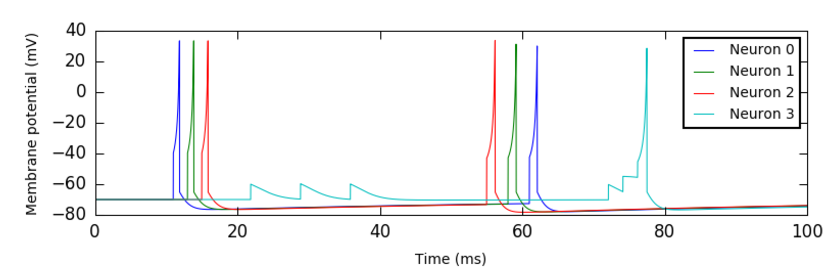
\includegraphics[width=4.0in]{SpikingExample.pdf}}
  \captionsetup{justification=centering, skip=3pt}
  \caption{Izhikevich Model Simulation \cite{Iz2005}\cite{carnevale2006neuron}}
  \label{fig:spiking example}
\end{subfigure}
\caption{Example Spiking Activation Function Model}
\label{fig:Example Spiking Model}
\end{figure}

To emulate complex behavior, the artifical neurons are connected in networks, typically with layers of sub-networks which are in affect separated by the non-linear activation function.
Examples of both rate-based and spiking artificial neural networks can be seen in \fref{fig:Rate-based Model Network} and \fref{fig:Spiking Model Network} respectively.
Typically neural networks process in a feed-forward fashion. Considering \fref{fig:Artificial Neural Network}, this means the input arrives on the left, the inputs propagate to neurons N0 through N3. WHen N0 through N3 are processed, their values propagate forward to neurons N4 and N5 etc.. SOmetime \ac{ann}s also include recursion where for example neurons N0 through N4 are not only influenced
by the input, but also by themselves. Many \ac{ann}s operate only in feed-forward fashion but some popular \ac{ann}s, such as Long short-term memory (LSTM), employ recursion.

Another popular \ac{ann} known as Deep Neural Networks (\ac{dnn}) have proved very popular over the last few years. They get good press in applications such as image recognition and speech recognition. 
Deep Neural Networks are often formed from tens of layers of \ac{an}s with each layer containing many \ac{an}s. \ac{dnn}s are also processed in a feed-forward manner with one layer being the inputs to the next layer. 
As mentioned \cite{krizhevsky2012imagenet}, these useful \ac{dnn}s often require hundreds of thousands of \ac{an}s and within the network, each \ac{an} can have hundreds, even thousands of feeder or pre-synaptic \ac{an}s.
There have been implementations that use different number formats from double precision floating point to eight bit integers, but in all cases these useful \ac{ann}s require a significant amount of memory to store the connection weights (parameters).


\begin{figure}[!t]
  % the [] contains position info e.g. [!t] means here
  \centering
  \captionsetup{justification=centering}
  \captionsetup{width=.9\linewidth}
  \begin{subfigure}{.9\textwidth}
    \centerline{
    \mbox{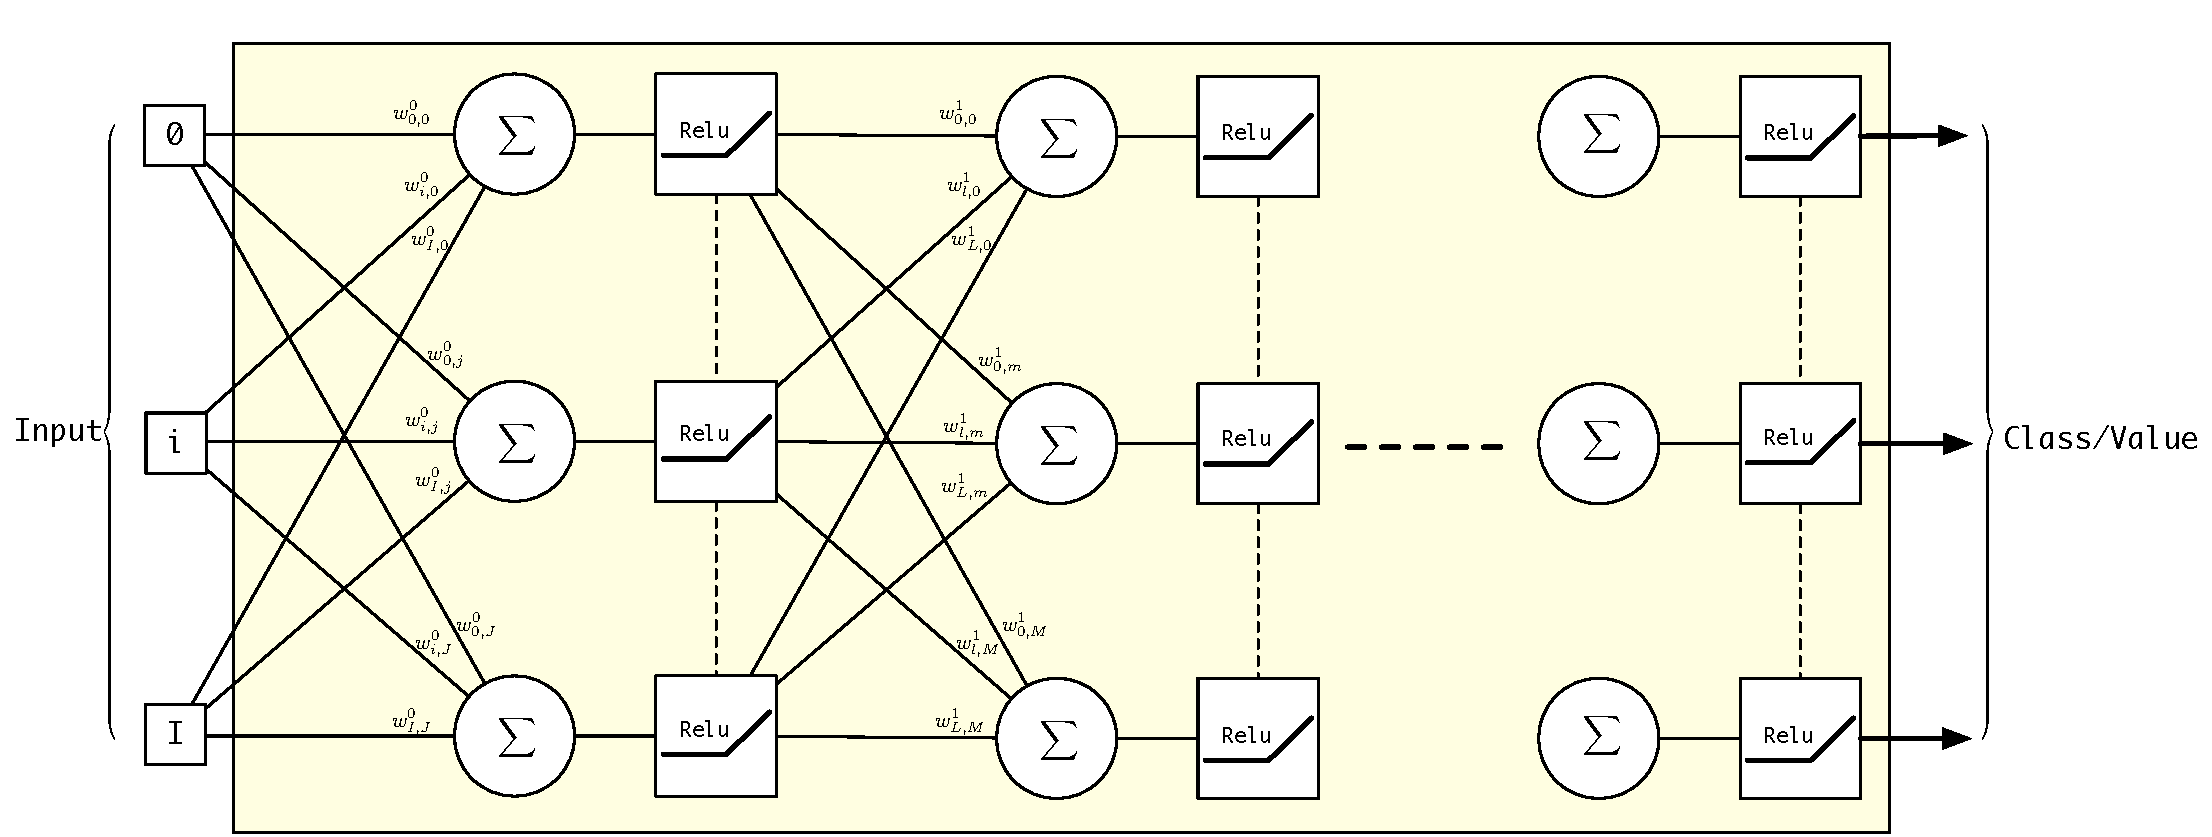
\includegraphics[width=0.85\textwidth]{RateBasedNeuralNetwork.pdf}}
    }
    \caption{Rate-based Model Artificial Neural Network (with ReLu activation function)}
    \label{fig:Rate-based Model Network}
  \end{subfigure}
  
  \begin{subfigure}{.9\textwidth}
    \centerline{
    \mbox{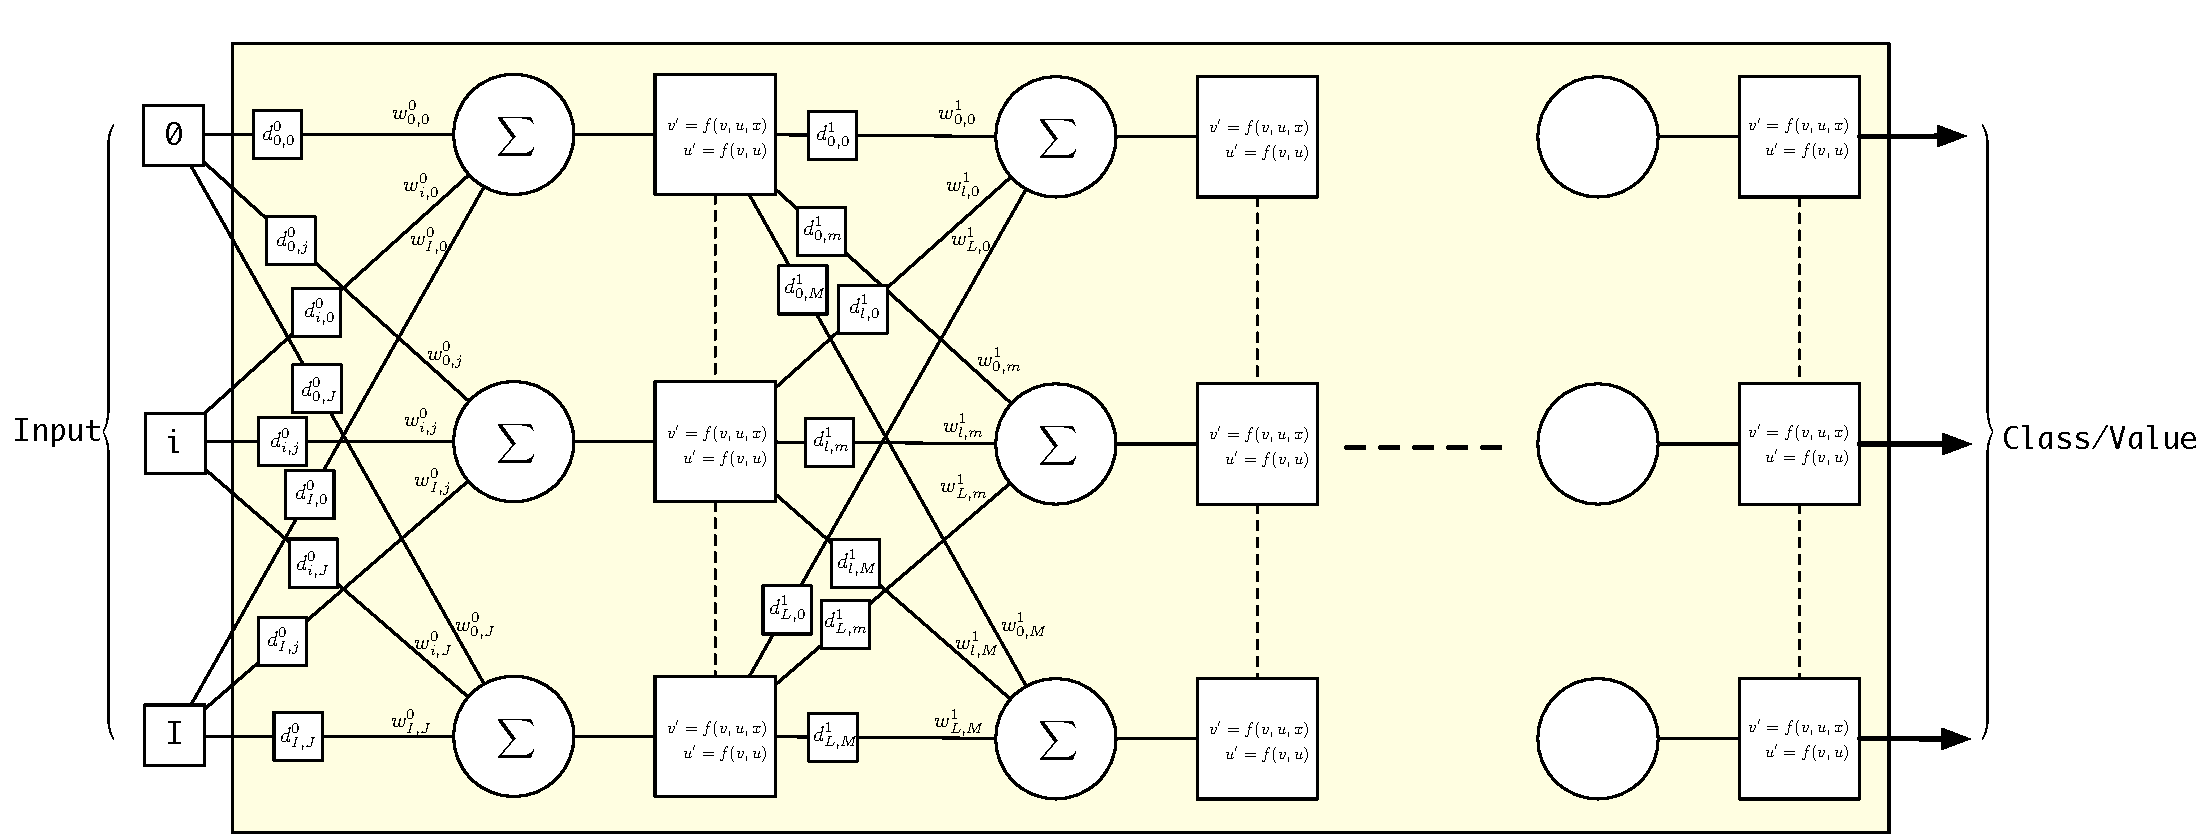
\includegraphics[width=0.85\textwidth]{SpikingNeuralNetwork.pdf}}
    }
    \caption{Spiking-based Model Artificial Neural Network}
    \label{fig:Spiking Model Network}
  \end{subfigure}
  \caption{Layered Artificial Neural Networks}
  \label{fig:Layered Artificial Neural Networks}
\end{figure}

Although the spiking neural network more closely models the behavior of real neurons, over the last 20 years there 
have been breakthroughs in the configuring of rate-based models especially with the introduction of the back-propagation
algorithm and stochastic gradient descent. Along with the abundance of data now available in the form of voice, images etc. to "teach" these networks
using back-propagation, most of the effective applications of artificial neural networks have employed these rate-based models.

\iffalse
Our research will focus on these rate-based models which we will now refer to as \ac{ann}s.
\fi

This work does not address the training of these rate-based \acp{ann}, the training is mostly performed offline. This work is addressing the inference of \acp{ann}.
During inference, the most computationally intensive operation is the multiply accumulate associated with the \ac{an} activation, which can involve hundreds or thousands of multiply-accumulates.
The \ac{an} activation calculation for the rate-based \ac{an} in figure \ref{fig:Rate Based Model} is shown in equation \eqref{eq:activation function}.

\begin{alignat}{2} 
\label{eq:activation function}
\text{\ac{an} Activation }\hspace{4mm} A & = f\bigg(\sum_{n=0}^{C_n}W_n \cdot A_n\bigg)  \\
              &\mathbf{C_p} \text{ is the number of pre-synaptic connections} \notag\\
              &\mathbf{W_p} \text{ is the weight of a connection} \notag\\
              &\mathbf{A_p} \text{ is the activation value of the pre-synaptic neuron} \notag \\
\text{and }   &f(x) \text{ is the activation function such as ReLu } \notag 
\end{alignat}

\section[ANN Layers Problem]{ANN Layers}
\label{sec:ANN Layers}

In figures \ref{fig:Network of ANs} and \ref{fig:Rate-based Model Network}, the \ac{ann} is shown to be constructed using layers of \acp{an}. It has long been known that a single layer of \acp{an} can be used linearly partition an n-dimensional input, as shown in figure \ref{fig:linear discrimination}.
However, if a more complex partition is required, this cannot be achieved using a single layer of \acp{an}. A higher order classification, as shown in figure \ref{fig:linear discrimination} can only be achieved using multiple layers of \acp{an}. 
In addition, to ensure the multiple layers cannot be mathematically collapsed into a single layer, the activation function $f(x)$, as shown in figure \ref{fig:Rate Based Model} must be a non-linear function.



\begin{figure}[h]
\centering
  \begin{subfigure}{.4\textwidth}
    \centering
    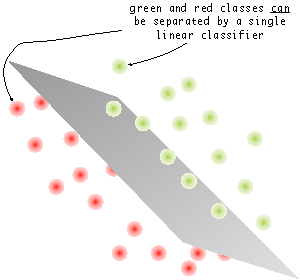
\includegraphics[width=0.85\textwidth]{linearDiscrimination}
    \captionsetup{width=.8\textwidth, justification=centering, skip=20pt}
    \caption{Linear Classification using a single layer}
    \label{fig:linear discrimination}
  \end{subfigure}%
  \begin{subfigure}{.4\textwidth}
    \centering
    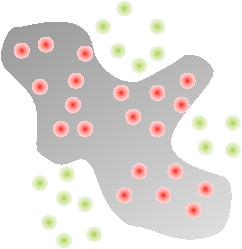
\includegraphics[width=0.7\textwidth]{complexDiscrimination}
    \captionsetup{width=.8\textwidth, justification=centering, skip=10pt}
    \caption{Complex Classification requires multiple layers}
    \label{fig:complex discrimination}
  \end{subfigure}
\captionsetup{justification=centering, skip=10pt}
\caption{Classification using \acp{ann} layers}
\label{fig:Discrimination}
\end{figure}


\subsection{Deep Neural Networks}
\label{sec:Deep Neural Networks}

As mentioned, a single layer of neurons can be used as a linear classifier as long as the classes can be separated using a linear function.
Even some simple cases cannot be linearly separated, an example often used is an exclusive-OR gate.

Even with a layered \ac{ann}, the final output comes from a single layer. To allow this final layer to linearly separate classes, the original input needs to be transformed into a space where the classes can be linearly separated.
\acf{dnn} are \acp{ann} that incorporate many layers of \acp{an}, often which are often up to tens of layers deep.
The additional layers are incorporated to translate the space of the input so the various classes being identified can be separated using linear classifiers in the later layers.

A recent very successful example of a \ac{dnn}, known as a \acf{cnn} was used to classify objects in images \cite{krizhevsky2012imagenet}.
These \acp{cnn} use the early layers to identify low-level features and later layers are used combine these features into yet more higher-level features.
Finally, the combination of high-level features are used to identify the required classes.
This layering is shown in \fref{fig:Deep network showing feature layers}.
\begin{figure}[h]
\centering
\includegraphics[width=0.95\textwidth]{deepNetworkBlockDiagram}
\captionsetup{justification=centering, skip=5pt}
\caption{Deep network showing feature layers}
\label{fig:Deep network showing feature layers}
\end{figure}

In figure \ref{fig:Deep network showing feature layers}, the final layer is often a fully connected linear classifier with the output representing the probability of a particular class being present in the image.
In practice, these \acp{dnn} can be used as classifiers or as function approximators.

\iffalse
In practice, useful deep neural networks are very large and often exceed the capacity of single GPUs. Therefore,  there is opportunity for a solution that provides
real-time acceleration and storage of of these systems.
\fi


\subsection{Feature Layers}
\label{sec:Feature Layers}

For the most part, different \acp{ann} are characterized by how the \acp{an} are interconnected and the activation function employed.

The typical \ac{dnn} layers are processed in a feed-forward fashion where the pre-synaptic \acp{an} are formed from \acp{an} in the previous layer.
There are some types of \ac{dnn} which also include recursive connections where the the pre-synaptic \acp{an} include \acp{an} from the current layer.
A popular recursive \ac{dnn} is \acf{lstm}. Although this work does not preclude supporting \ac{lstm} in the future, the focus of this work is on the feed-forward type \ac{dnn}.

As described in \ref{sec:Deep Neural Networks}, a \ac{dnn} layer transforms the previous layer with each higher layer providing a coarser grained transformation. This is best seen in image recognition application were the early layers identify low level shapes or features, such as angled lines with higher layers identifying higher order shapes such as circles, blocks etc. 
Although the image recognition applicaition is somewhat intuitive, it is believed that in less intuitive applications the \ac{dnn} performs a similar fine to coarse feature extraction.

The connections between layers can be locally-connected or fully-connected. 
With locally-connected layers (see figure \ref{fig:Locally-Connected Interconnects}), a particular layer \acp{an} pre-synaptic \acp{an} are formed from regions of the previous layer.
With fully-connected layers (see figure \ref{fig:Fully-Connected Interconnects}), a particular layer \acp{an} pre-synaptic \acp{an} are formed from all \acp{an} in the previous layer.
In many cases, a \ac{dnn} is constructed with lower layers being locally-connected and higher layers being fully connected.

\begin{figure}[h]
\centering
  \begin{subfigure}{.4\textwidth}
    \centering
    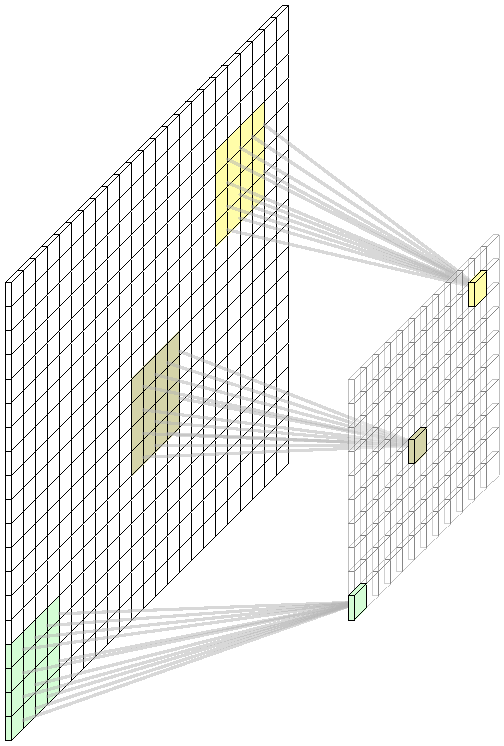
\includegraphics[width=0.65\textwidth]{locallyConnectedInterconnects}
    \captionsetup{width=.8\textwidth, justification=centering, skip=10pt}
    \caption{Locally-Connected Interconnects}
    \label{fig:Locally-Connected Interconnects}
  \end{subfigure}%
  \begin{subfigure}{.4\textwidth}
    \centering
    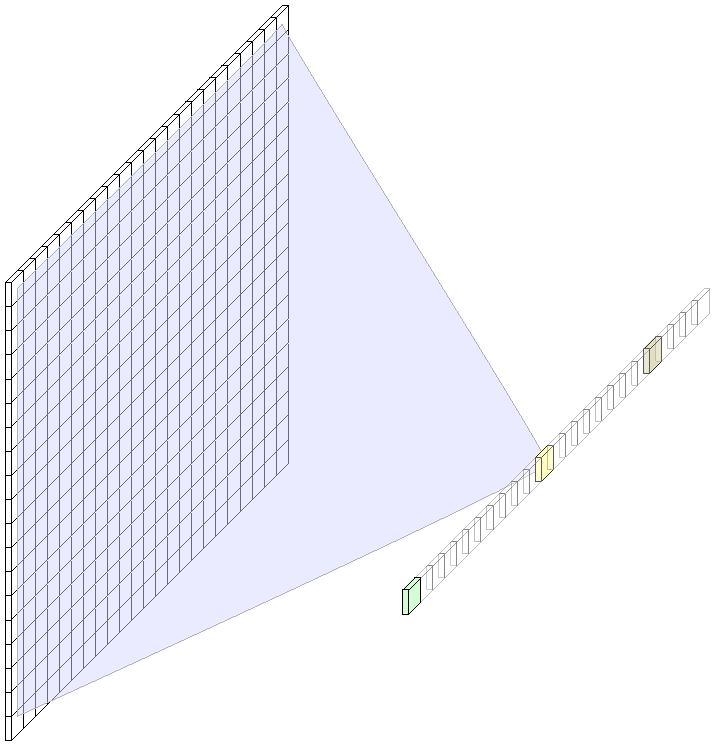
\includegraphics[width=0.85\textwidth]{fullyConnectedInterconnects}
    \captionsetup{width=.8\textwidth, justification=centering, skip=10pt}
    \caption{Fully-Connected Interconnects}
    \label{fig:Fully-Connected Interconnects}
  \end{subfigure}
\captionsetup{justification=centering, skip=10pt}
\caption{Layer Connection Types}
\label{fig:Layer Connection Types}
\end{figure}

With locally-connected layers, the pre-synaptic \acp{an} connection weights are often formed from identifying particular features. In early uses of locally-connected \acp{ann}, the first layers weights were often hand-generated. With automatically trained \acp{ann}, the feature detectors at each layer are often created during training.
With image recognition \acp{ann}, the lower level features generated during automatic training are often intuitive and are trained to detect small features such as lines at various angles, different curves etc..
In the general case, the trained feature detectors may not be as intuitive.
Some contrived examples of locally-connected feature detectors are shown in figure \ref{fig:Features and locally-connected filters (kernels)}.
\begin{figure}[h]
\centering
  \begin{subfigure}{.7\textwidth}
    \centering
    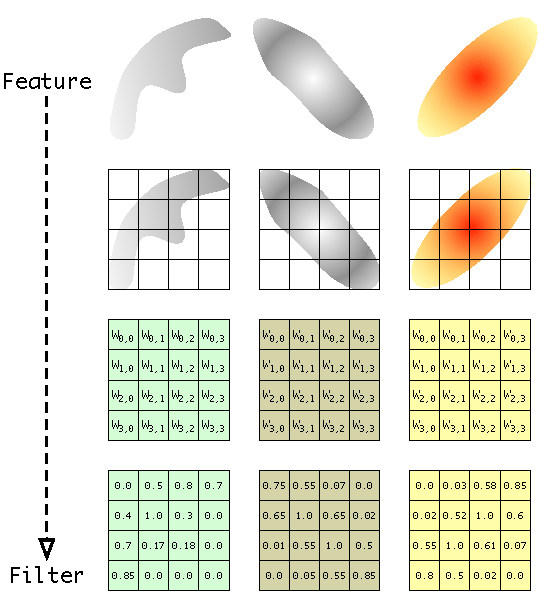
\includegraphics[width=0.65\textwidth]{locallyConnectedFeatures}
    \captionsetup{justification=centering, skip=5pt}
    \caption{Features and locally-connected filters (kernels)}
    \label{fig:Features and locally-connected filters (kernels)}
  \end{subfigure}%

\bigskip

  \begin{subfigure}{.7\textwidth}
    \centering
    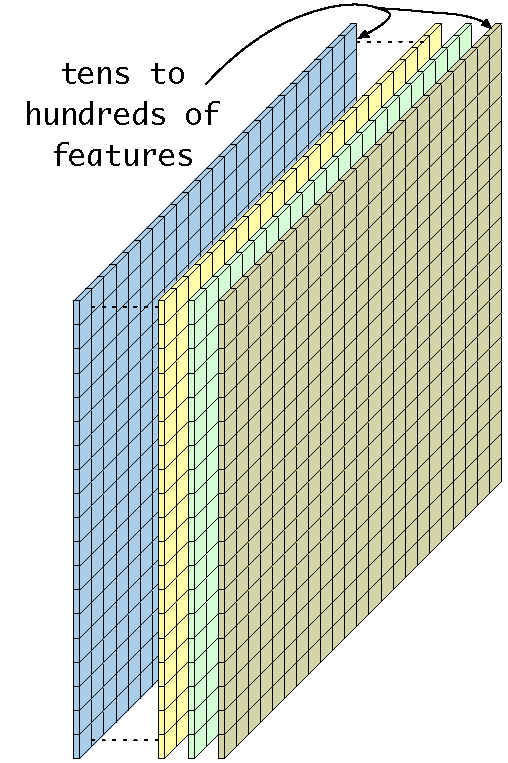
\includegraphics[width=0.45\textwidth]{layer3DFeatures}
    \captionsetup{justification=centering, skip=5pt}
    \caption{3D layers of Features}
    \label{fig:3D layers of Features}
  \end{subfigure}
\captionsetup{justification=centering, skip=10pt}
\caption{Layer Feature Planes}
\label{fig:Layer Features}
\end{figure}

%%\begin{figure}[h]
%%\centering
%%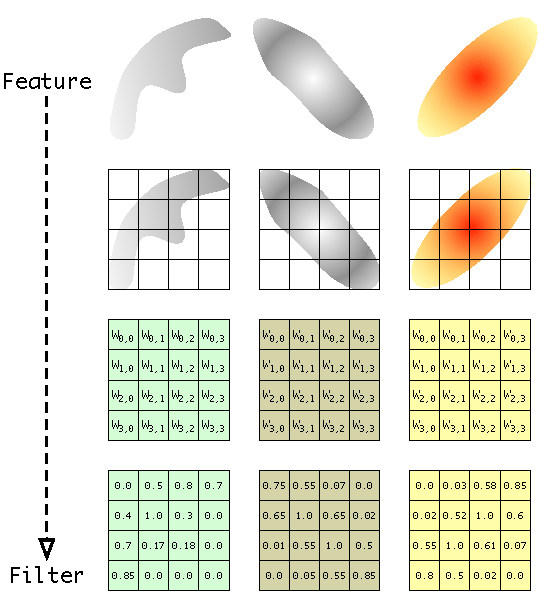
\includegraphics[width=0.55\textwidth]{locallyConnectedFeatures}
%%\captionsetup{justification=centering, skip=5pt}
%%\caption{Features and locally-connected filters (kernels)}
%%\label{fig:Features and locally-connected filters (kernels)}
%%\end{figure}
%%
%%\begin{figure}[h]
%%\centering
%%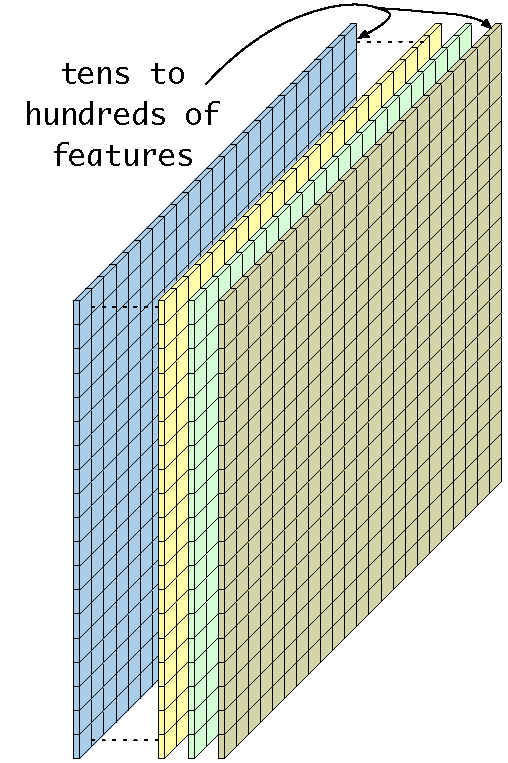
\includegraphics[width=0.55\textwidth]{layer3DFeatures}
%%\captionsetup{justification=centering, skip=5pt}
%%\caption{Features form 3D layers}
%%\label{fig:Features form 3D layers}
%%\end{figure}

These locally-connected layers have multiple filters applied to the same region-of-interest in the previous layer. The next layer therefore becomes a 3D array with the Z-axis representing the features. 
The number of feature filters applied at each layer can be tens to hundreds of filters.
The filters operating on these 3D layers are themselves 3D and therefore the number of weights associated with each filter is usually hundreds to thousands of weights. 

The feature kernels employed in the locally-conencted layers can be unique to the regions of the previous layer or the same filter kernels can be employed across the entire previous layer.
In the case of employing the same kernels across the entire input layer the \ac{ann} is known as a \acf{cnn}. The \acp{cnn} are examples of \acp{ann} which can take advantage of reuse described in \ref{sec:chap-one}. 
These \acp{cnn} can store the filter kernels in local \ac{sram} and construct an entire feature plane. These \acp{cnn} can be considered a subset of the generic case of \ac{dnn} where the kernels can be unique across the entire input layer.
This work considers the more generic \ac{dnn} case and supports acceleration of both \acp{dnn} and the subset \acp{cnn}.

An example of a \ac{cnn} can be seen in figure \ref{fig:Example DNN} with the layer configurations shown in table \ref{tab:Layer Configuration}. A \ac{cnn} similar to this has demonstrated high levels of efficacy in image recognition applications.
{\textbf{\textcolor{black}{Therefore, this work will use this particular \ac{dnn} as a template for estimating the storage and processing requirements and the range of pre-synaptic fanins.}}}

%%
\iffalse
\begin{table}[ht]
\centering
\begin{tabular}{|c|c|c|c|c|c|c|c|}\cline{3-8}
\multicolumn{2}{c|}{\multirow{2}{*}{}}&\multicolumn{3}{c|}{Singular}&\multicolumn{3}{c|}{Plural}\\\cline{3-8}
\multicolumn{2}{c|}{}&Neuter&Masculine&Feminine&Masculine&Feminine&Neuter\\\hline
\multicolumn{1}{|c|}{\multirow{2}{*}{I}}&Inclusive&\multicolumn{3}{|c|}{\multirow{2}{*}{O}}&\multicolumn{3}{c|}{X}\\\cline{2-2}\cline{6-8}
&Exclusive&\multicolumn{3}{c|}{}&\multicolumn{3}{c|}{X}\\\hline
\multirow{2}{*}{II}&Informal&\multicolumn{3}{|c|}{X}&\multicolumn{3}{c|}{X}\\\cline{2-8}
&Formal&\multicolumn{6}{|c|}{X}\\\hline
\multirow{2}{*}{III}&Informal&\multicolumn{1}{c|}{\multirow{2}{*}{O}}&X&X&\multicolumn{2}{|c|}{X}&\multicolumn{1}{c|}{\multirow{2}{*}{O}}\\\cline{2-2}\cline{4-7}
&Formal&&\multicolumn{4}{|c|}{X}&\\\hline

\end{tabular}
\end{table}
\fi

\begin{sidewaysfigure}[h]
  %\begin{adjustbox}{angle=0, width=1.0\textwidth}
    \centering
    \captionsetup{justification=centering}
    \begin{subtable}{.9\textwidth}
      %\captionsetup{justification=centering, skip=-5pt}
      \centering
      %\begin{center}
       % [lr] ~ left align col 0 and right align col 1
       % e.g. 4 columns could be lccr
      \begin{adjustbox}{width=1\textwidth}
        \begin{tabular}{|r|c|c|c|c|c|c|c|c|c|c|c|c|c}\cline{3-13}
          %\toprule
           \multicolumn{2}{c|}  {\multirow{2}{*}{}}    & \multicolumn{11}{c|}{Layers}    \\\cline{3-13}
           \multicolumn{2}{c|}{}                       &  1 & 2 & 3 & 4 & 5 & 6 & 7 & 8 & 9 & 10 & 11  \\\cline{3-13} \cline{1-13}
           \multicolumn{2}{|r|}{Type}                  &  Input          & Locally      & Pooling           & Locally             & Pooling             & Locally             & Locally             & Locally             &  Fully              &  Fully                 &  Fully         &                                    \\\cline{1-13}
           \multirow{3}{*}{Dimensions}               &X& \num{       256}& \num{     55}& \num{    27}      & \num{     27}       & \num{     13}       & \num{     13}       & \num{     13}       & \num{     13}       & \num{      4096}    & \num{     4096}        & \num{    1024} &                                    \\
                                                     &Y& \num{       256}& \num{     55}& \num{    27}      & \num{     27}       & \num{     13}       & \num{     13}       & \num{     13}       & \num{     13}       & \num{         1}    & \num{        1}        & \num{       1} &                                    \\
                                                     &Z& \num{         3}& \num{     96}& \num{    96}      & \num{    256}       & \num{    256}       & \num{    384}       & \num{    384}       & \num{    256}       & \num{         1}    & \num{        1}        & \num{       1} &                                    \\\cline{1-13}
           \multirow{3}{*}{Filter Dimensions}        &X&    na           & \num{     11}& \num{     2}      & \num{      5}       & \num{      2}       & \num{      3}       & \num{      3}       & \num{      3}       & \num{        13}    & \num{     4096}        & \num{    4096} &                                    \\
                                                     &Y&    na           & \num{     11}& \num{     2}      & \num{      5}       & \num{      2}       & \num{      3}       & \num{      3}       & \num{      3}       & \num{        13}    & \num{        1}        & \num{       1} &                                    \\
                                                     &Z&    na           & \num{      3}& \num{     1}      & \num{     96}       & \num{      1}       & \num{    256}       & \num{    384}       & \num{    384}       & \num{       256}    & \num{        1}        & \num{       1} &                                    \\
            \multicolumn{2}{|r|}{Stride           }    &    na           & \num{      4}& \num{     2}      & \num{      2}       & \num{      2}       & \num{      1}       & \num{      1}       & \num{      1}       &              na     &             na         &            na  &                                    \\\hline
            \multicolumn{2}{|r|}{Pre-synaptic Fanin}   &    na           & \num{    363}& \num{     4}      & \num{   2400}       & \num{      4}       & \num{   2304}       & \num{   3456}       & \num{   3456}       & \num{     43264}    & \num{     4096}        & \num{    4096} & \multicolumn{1}{c|}{Total        } \\\cline{14-14}
            \multicolumn{2}{|r|}{Number of \ac{an}}    & \num{    196608}& \num{ 290400}& \num{ 69984}      & \num{ 186624}       & \num{  43264}       & \num{  64896}       & \num{  64896}       & \num{  43264}       & \num{      4096}    & \num{     4096}        & \num{    1024} & \multicolumn{1}{c|}{\num{ 969152}} \\
            \multicolumn{2}{|r|}{Number of Weights}    &    na           & \num{  34848}& na                & \num{ 614400}       & na                  & \num{ 884736}       & \num{ 1327104}      & \num{ 884736}       & \num{ 177209344}    & \num{ 16777216}        & \num{ 4194304} & \multicolumn{1}{c|}{\num{ 2.02e8}} \\\hline
        \end{tabular}
      \end{adjustbox}
      \captionsetup{justification=centering, skip=9pt}
      \vspace{0.5cm}
      \caption{Layer Configuration \cite{krizhevsky2012imagenet}}
      \label{tab:Layer Configuration}
      %  \end{center}
    \end{subtable}
  
    \bigskip

    %\begin{adjustbox}{width=1.0\textwidth}
      \begin{subfigure}{1\textwidth}
        \centering
        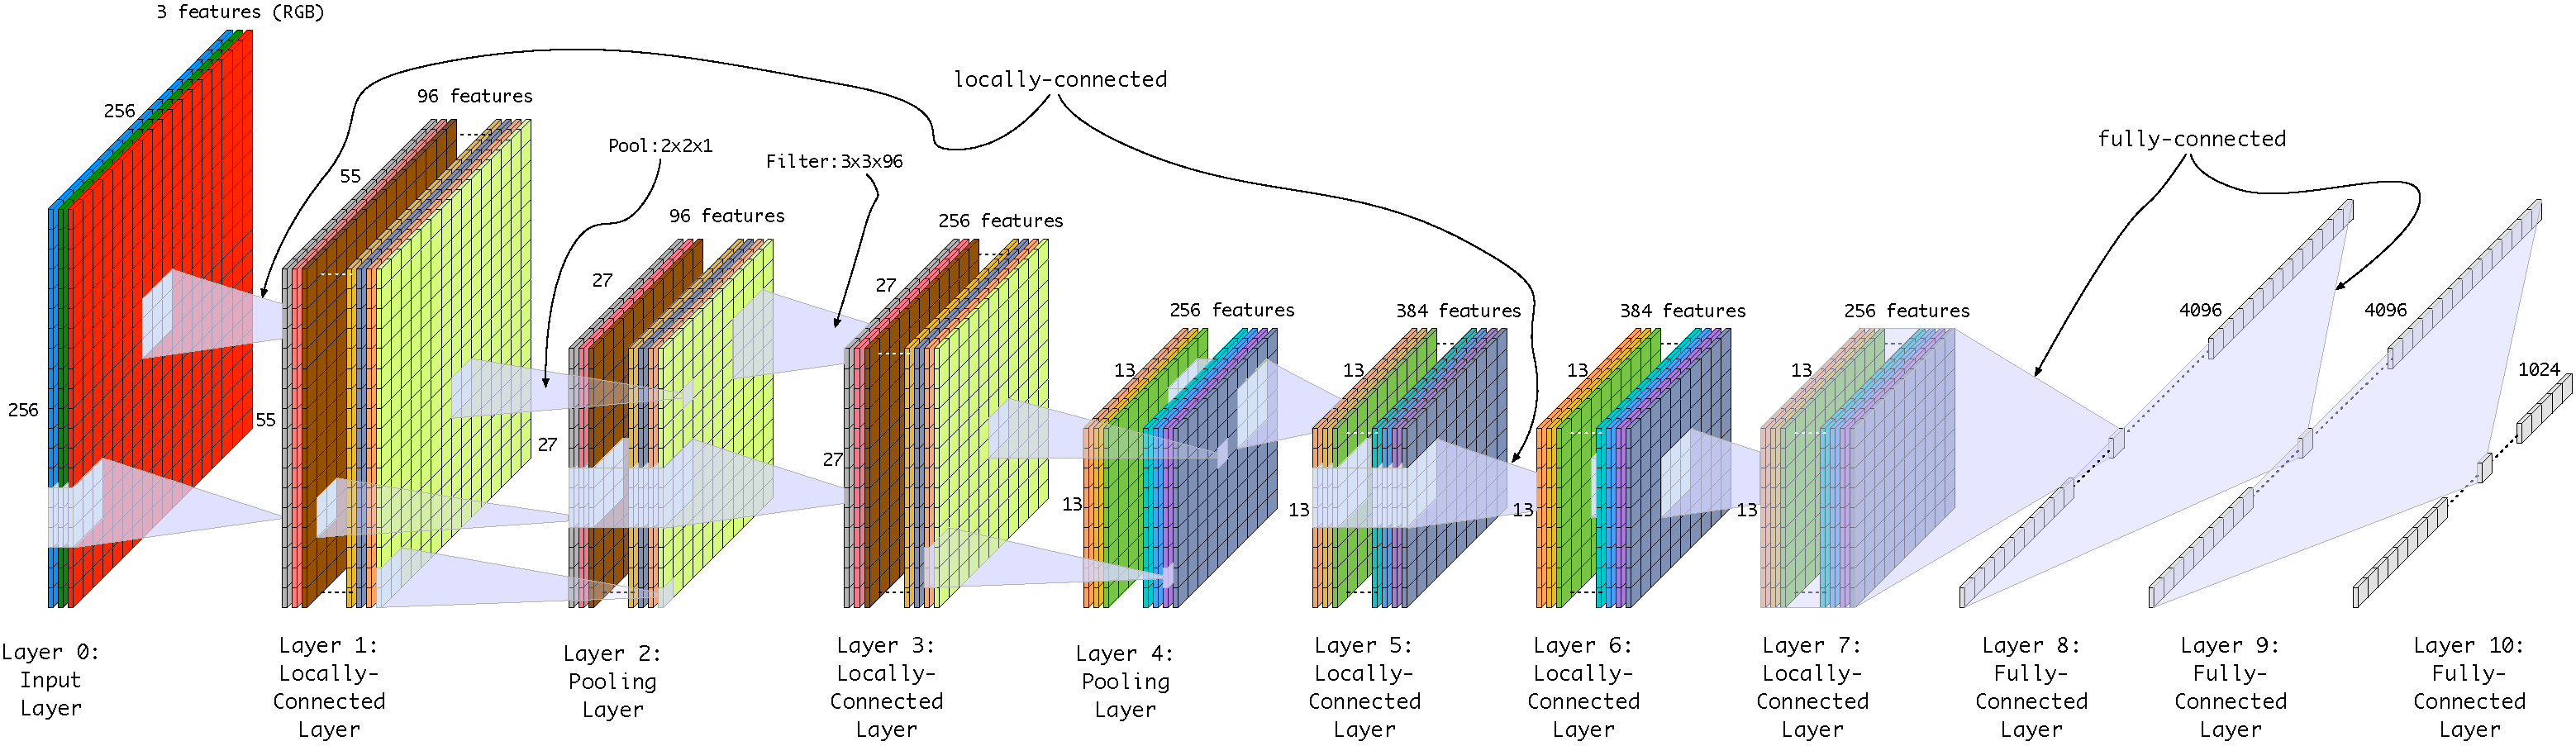
\includegraphics[width=1.0\textwidth]{fullDNN}
        \captionsetup{justification=centering, skip=15pt}
        \caption{Example DNN \cite{krizhevsky2012imagenet}}
        \label{fig:Example DNN}
      \end{subfigure}
    %\end{adjustbox}
  
  %\end{adjustbox}
  \caption{Typical DNN\cite{krizhevsky2012imagenet}}
  \label{fig:Typical DNN}
\end{sidewaysfigure}



\iffalse
\begin{sidewaysfigure}[h]
\centering
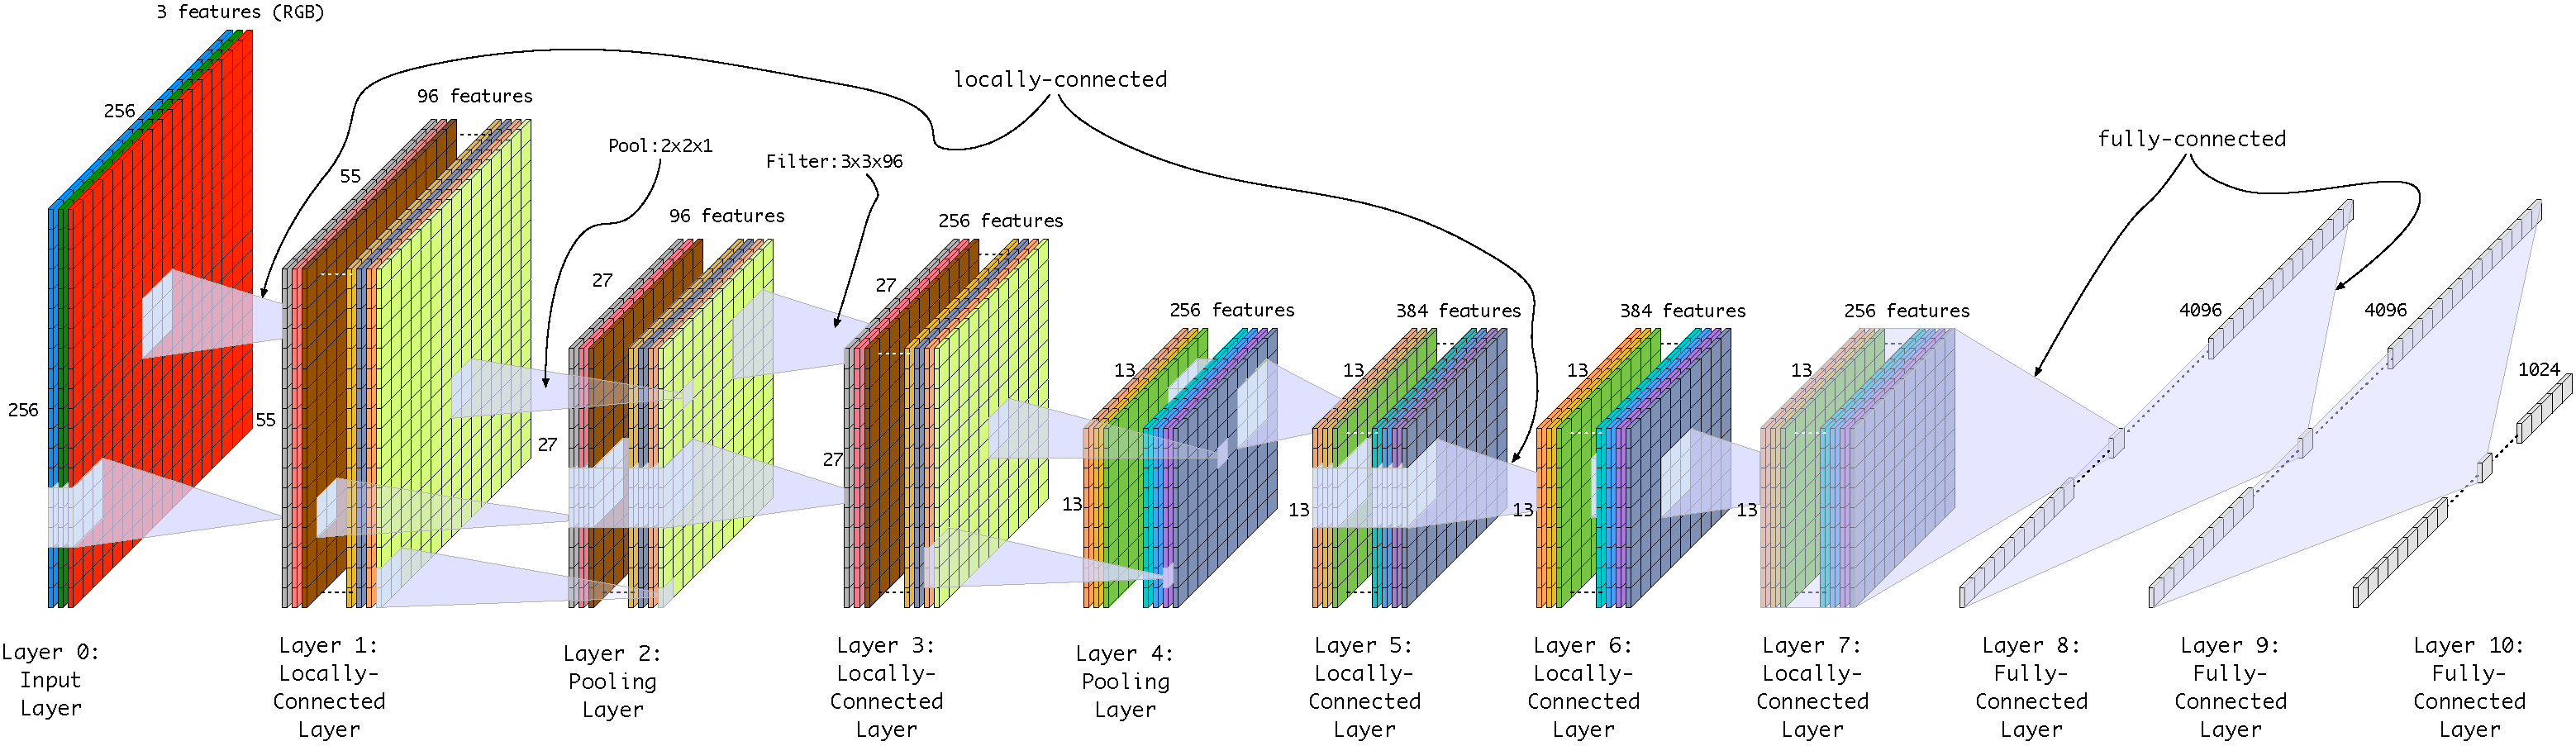
\includegraphics[width=1.0\textwidth]{fullDNN}
\captionsetup{justification=centering, skip=15pt}
\caption{Example DNN \cite{krizhevsky2012imagenet}}
\label{fig:Example DNN}
\end{sidewaysfigure}
\fi


\section[The Problem]{The Problem}
\label{sec:The Problem}

To approach the capabilities observed in human behavior, such as object recognition these \ac{ann}s become very large.
They often utilize hundreds of thousands of neurons to implement what a human would consider a relatively straightforward task.
For example, a "useful" \ac{ann} similar to that described in \cite{krizhevsky2012imagenet} that is used to recognize up to 1000 different object classes, has a network size of approximately 650,000 neurons and 630 million synaptic connections \cite{krizhevsky2012imagenetPreso}. 

The increased performance of \ac{ann}s over classical methods in image recognition and voice recognition might suggest that \ac{ann}s might out-perform techniques in other applications.
There is reason to believe that \acp{ann} will replace existing control and monitoring functions in existing systems.

If \ac{ann}s fulfill their potential, systems employing \ac{ann}s will utilize them for various functions, such as engine monitoring, anomaly detection, navigation etc. all within the same system.
Considering the various functions a complex customer facing or edge application system performs, it is likely that many real-world applications will employ multiple disparate instances of these useful sized \ac{ann}s.
Assuming these complex functions will require \ac{ann}s similar in size to \cite{krizhevsky2012imagenet}, these implementations will be processing multiple large \ac{ann}s at or near real-time.

Considering the storage required for the input, the \ac{an} states and most significantly the weights for each of the \ac{an}s, the storage requirements results in gigabytes of memory.
When these \ac{ann}s are required to be solved in fractions of a second, the processing and memory bandwidth becomes prohibitive.

\subsection[ANN Processing]{ANN Processing}
\label{sec:ANN Processing}
As a metric, this work assumes that any useful \ac{ann} will employ 100s of thousands of \ac{an}s. Although there is a lot of debate regarding number formats for \ac{ann}s, this work also assumes single-precision floating point.
Assuming an \ac{ann} with 250K neurons and an average fanin to each \ac{an} of 2000, a system employing 10 \ac{ann}s for various disparate functions and an average processing time of \SI{10}{\milli\second} suggests a average bandwidth of \SI[per-mode=symbol]{16}{\tera \bit \per \second} (see equation \ref{eq:averageBandwidth}).

% {2} means 2 columns
\begin{alignat}{2} 
  \label{eq:averageBandwidth}
  \text{Average }\text{Bandwidth} & = \sum_{\mathbf{n}=0}^{\bar{\mathbf{N_n}}}\big(\frac{\Bar{\mathbf{N_a}}\cdot \Bar{\mathbf{C_p}} \cdot \bar{\mathbf{b_w}}}{\bar{\mathbf{T_p}}} \big) \notag  \\
  & = \sum_{\mathbf{n}=0}^{9}\big(\frac{\num{250d4} \cdot \num{2d3} \cdot 32}{\num{10d-3}} \big) \notag \\
  & = \SI[per-mode=symbol]{16}{\tera\bit\per\second} \\
  \text{where } &\mathbf{N}_n \text{ is the number of \ac{ann}s} \notag\\
                &\mathbf{N}_a \text{ is the average number of \ac{an}s} \notag\\
                &\mathbf{C_p} \text{ is the average number of connections} \notag\\
  \text{and }   &\mathbf{T_p} \text{ is the processing time} \notag
\end{alignat}

Therefore, when implementing \ac{ann}s, the memory requirements are significant. The storage is required for the input, the \ac{an} state and most significantly the weights for each of the \acp{an} pre-synaptic connections. This storage requirement often results in gigabytes of memory.

In addition, in edge applications, it is anticipated that these \ac{ann}s will be required to be solved in fractions of a second, in which case the processing and memory bandwidth becomes prohibitive.

The problem becomes \hyphenquote{american}{\textbf{\textcolor{black}{to provide deterministic at or near real-time performance within tolerable power and space constraints for edge systems employing inference on multiple disparate useful-sized neural networks.}}}
%\hlc[gray]{hello}

Considering that \ac{dram} is required to store the \ac{ann} parameters, why is it that much of the \ac{asic} and \ac{asip} \ac{ann} research employs \ac{sram} as an intermediate store? Well, in practice there are benefits if you can operate solely out of \ac{sram}.
Certainly good performance and potentially low power.
But use of \ac{sram} makes assumptions on the type of \acp{ann} that can be supported and the application in which the \ac{ann} is being deployed.
The primary requirement of the type of \ac{ann} and the deployed application to allow effective use of \ac{sram} is "reuse". Reuse means that once parameters are transferred and stored in \ac{sram}, these parameters can be reused such that the \ac{sram} isn't simply an intermediate memory but something akin to a cache.

In some \ac{ann}s there are reuse opportunities. A prime example is \acp{cnn}, where the connection weights are reused. In \acp{cnn}, a common filter is passed across an input to form the next layer. These filter "kernels" can be held in memory and the input is read from \ac{dram} thus reducing the \ac{dram} bandwidth.
Even with \ac{dnn}s where weights may not be reused, when implementing multiple \ac{dnn}s, there is opportunity to hold the input in memory.
If the system is being employed in cloud applications or in training, there is opportunity to reuse inputs whilst performing batch processing.

But \ac{sram} comes at a price, its big. Often when we see physical layouts of NN processors, they are dominated by the silicon area of the \ac{sram}. The area required for \ac{sram} has been understood for quite some time and companies attempt to create custom \acp{sram} to minimize the area impact.

So the question becomes, can a system employ \ac{dram} with minimal \ac{sram} and still provide a high performance system within acceptable area constraints?

\iffalse
We believe a system can be designed with \ac{dram} as the primary processing store. This will require careful use of data structures to describe storage within \ac{dram} to ensure we make good use of the potential bandwidth. But there are other benefits we will take advantage of, but more about that later.
\fi

\iffalse
There important application is disparate \ac{ann}s because specifically a form of \ac{dnn}, Convolutional Neural networks (\ac{cnn}) have gotten good press recently, but they are not the only \ac{dnn}.
\fi

Even in cloud applications, there are limitations on reuse. We paraphrase a quote from a Google paper \cite{tensorflow2015-whitepaper} on their Tensor Processing Unit ASIC (TPU):

\hyphenquote{american}{the architecture research community is paying attention to NNs, but of all the papers at ISCA 2016 on hardware accelerators for NNs, alas, all nine papers looked at \ac{cnn}s, and only two mentioned other NNs. Unfortunately \ac{cnn}s represent only about 5\% of our datacenter NN workload}

The applications targeted by the google TPU \cite{tensorflow2015-whitepaper} assume multiple requests, so reuse in the form of batch processing is still of great benefit, but the bulk of the requests in \cite{tensorflow2015-whitepaper} are fully-connected \ac{dnn}s and in these cases weight reuse is not as benefitial and the performance of the TPU is degraded when implementing these fully-connected \ac{dnn}s.

Therefore, implementations that focus on \ac{cnn}s can suffer from severe degradation in performance when targeting generic types of \ac{ann}, such as locally and fully connected \ac{dnn}s and LSTMs.

This work focuses on edge applications employing disparate \ac{ann}s and assumes both weight reuse and batch processing do not apply.
Considering systems will want to perform multiple \ac{dnn}s simultaneously suggests that these edge systems will require usable memory bandwidth of the order of 10s of \SI[per-mode=symbol]{}{\tera \bit \per \second}.

In these cases, \textbf{\textcolor{black}{\ac{dram} bandwidth is the bottleneck}}.




\iffalse
So considering the performance improvements observed in other applications, it is expected that many customer facing or edge applications will implement multiple instances of artificial neural networks to perform various functions.
have very large memory and processing requirements.
require multiple instances of \ac{ann}s of similar size to the \ac{ann} described in \cite{krizhevsky2012imagenet}.

For example employing multiple cameras or monitoring and controlling different systems in a drone, a automobile each with an image recognition \ac{ann}\cite{krizhevsky2012imagenet}\cite{bojarski2016end} for navigation, engine monitoring along with other system control.
\fi

Some might suggest the requirements of these applications would be satisified by employing multiple graphics processor units(GPU).
In fact, Graphics processing Units (GPU) are used to implement large \ac{ann}s and in some \ac{ann} architectures, such as Convolutional NNs (\ac{cnn}), they are quite effective. However, we should not forget they are not optimized purely for \ac{ann} processing and are restricted by available SRAM and they are power hungry. These limitations will limit the effectiveness of GPUs regardless of what we might hear from the GPU community.
Even in the case of newer GPUs which are employing 2.5DIC technology, the memory bandwidth will still be limited by available \ac{dram} tecnology.
For example, a 2.5D solution employing High bandwidth Memory (HBM) would be limited to a maximum raw bandwith of the order of \SI[per-mode=symbol]{4}{\tera \bit \per \second}.
Also, its has proven very difficult, if not impossible to take advantage of the available memory bandwidth \cite{farabet2011neuflow} \cite{tensorflow2015-whitepaper}.
Given these multiple GPU systems have high real-estate and power requirements and given each instance consumes of the order of \SI{100}{\watt} to \SI{200}{\watt}.
Overall GPUs have limited suitability to meet edge application requirements.


Much of the \ac{ann} application specific (ASIC/ASIP) research has focused on taking advantage of the performance and ease of use of Static Random Access Memory or \ac{sram}. 
These implementations can be shown to be effective with specific \ac{ann} architectures (\ac{cnn}), server applications or the "toy examples" but when a system requires multiple disparate \ac{ann}s in an edge application, these implementations do not provide the required flexibility, storage capacity and deterministic performance.

How this work addresses the problem are outlined in section \ref{chap-five}.


%%---------------------------------------------------------------------------------------------------------
%%---------------------------------------------------------------------------------------------------------



%% Lee
%% In dissertation, change section* to chapter and subsection* to section


\chapter{Three-Dimensional Integrated Circuits (3DIC)}
\label{chap-three}

Over the last couple of decades, the ever shrinking world of \acp{ic} has enabled the introduction of devices society takes for granted such as personal computing and cell phones.

As \ac{ic} technology has shrunk, design complexity has grown to take advantage where hundreds of millions of transistors are placed on a typical \ac{ic}.
These \acp{ic} have evolved from performing small functions to becoming systems on a chip.

However, at some point, an \ac{ic} has to interface with another function and often that communication involves the moving of data to and from memory and the increase in complexity often drives a need for higher memory data bandwidth. 

The \ac{ic} complexity has been doubling approximately every two years but the external interfaces are restricted by physical limitations.
Within the \ac{soc}, the designer can take advantage of very wide interfaces, often thousands of bits wide to increase bandwidth, but when data is moved to off-chip memory, the widest buses are usually hundreds of bits wide.

One way to avoid this limitation is to employ \ac{3dic} (see figure \ref{fig:3DIC Die}). The advantages of \ac{3dic} are well understood. reducing the amount of off-chip communication increases bandwidth and reduces power. The power reduction comes from not having to drive the relatively
high capacitance inputs and outputs.

\begin{figure}
\centering
\begin{subfigure}{.8\textwidth}
  \centering
  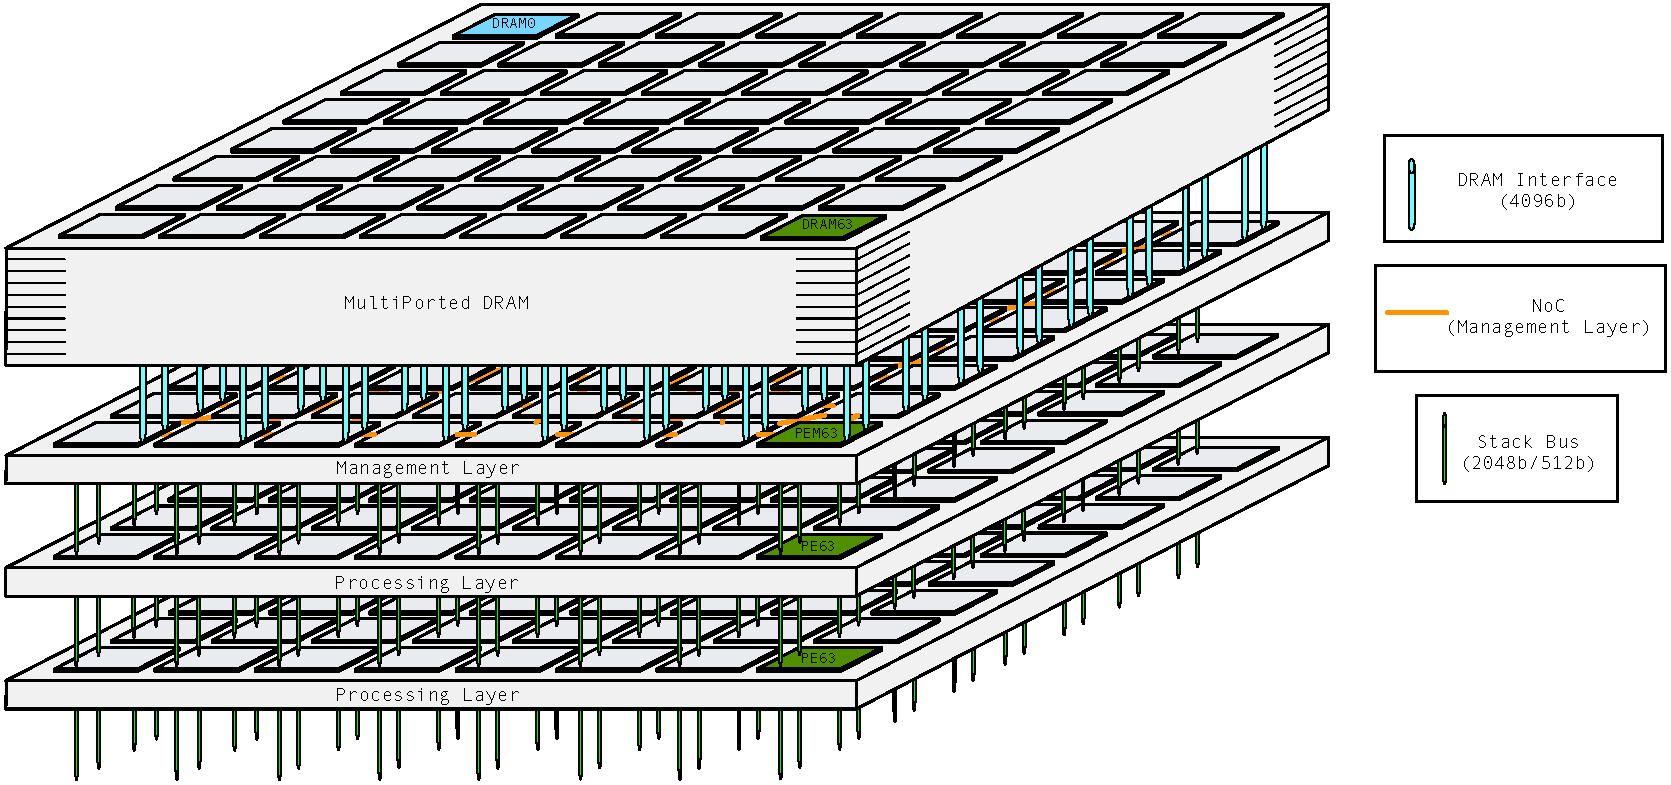
\includegraphics[width=1\textwidth]{DieStack}
  \captionsetup{justification=centering, skip=5pt}
  \caption{Different Die types stacked mounted on an interposer/package substrate}
  \label{fig:Die Stack}
\end{subfigure}%

\bigskip

\begin{subfigure}{.8\textwidth}
  \centering
  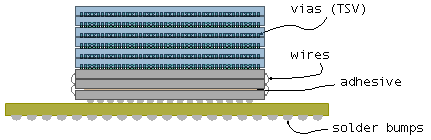
\includegraphics[width=1\textwidth]{DieStackConnections}
  \captionsetup{justification=centering, skip=5pt}
  \caption{Connection Types}
  \label{fig:Die Stack Connection Types}
\end{subfigure}
\captionsetup{justification=centering, skip=12pt}
\caption[3DIC Stack of Die]{3DIC Stack of Die}
\label{fig:3DIC Die}
\end{figure}

Taking advantage of \ac{3dic} means stacking die on top of one another and making connections directly between the die. These connections can be in the form of wire made at the edges of the die or using vias buried in the die itself.


Below is a summary the benefits of \ac{3dic} :
\begin{outline}
  \1 Reduced Power
    \2 mainly from not having to drive external outputs and receiving external inputs
  \1 Increased Connectivity
    \2 maintaining very wides buses through the \ac{soc} increases bandwidth
  \1 Ability to mix heterogeneous technology
    \2 Mixed Analog/Digital
    \2 Mixing memory technology and logic technology
  \1 Increase density and mitigation against the slowing of Moores Law
    \2 using the vertical domain to increase perceived transistor per $mm^2$
  \1 Potentially lower costs by combining simpler die rather than build a large die
    \2 yield benefits from combining higher yield die
  \1 Possibility of novel architectures \cite{Kim2016}
\end{outline}

Some disadvantages of \ac{3dic} are:
\begin{outline}
  \1 Reliability
  \1 Cost
    \2 being a relatively new technology it is still expensive 
    \2 \ac{tsv} technology is still unreliable
\end{outline}

There is still some reluctance to fully embrace \ac{3dic} but undoubtly the various barriers will be broken down.

The ability to mix heterogenous technology is of particular interest to this works target application because mixing technology targeted toward \ac{dram} with cmos logic technology is a heterogenous mix of which this work takes advantage.

In \cite{itrs2015_interconn} there are four definitions of \ac{3dic} interconnects:

\begin{outline}
%\section{3D-Wafer level package \cite{itrs2015_interconn}}
%\label{sec:3D-Wafer level package}

  \1 3D-Wafer level package \cite{itrs2015_interconn}
    \2 In this case, different die are stacked and then connected using traditional bond bumps and/or bond wires at the periphery of the chip.
    \2 This technique provides better transistor density compared to traditional 2D-IC with improvements in interconnect density.

%\section{3D-Stacked SoC\ac{soc} \cite{itrs2015_interconn}}
%\label{sec:3D-Stacked \ac{soc}}
  \1 3D-Stacked \ac{soc} \cite{itrs2015_interconn}
    \2 In this case, different die are stacked and then connected using \acp{tsv}. The \acp{tsv} connect the dies to intermediate metal layers known as global metal layers. This allows the indivial die to maintain a high level of functionality and thus is similar to connecting functional building blocks meaning the individual die are likely to be significant functional pieces of \ac{ip}.
    \2 using \acp{tsv} provides a medium level of interconnect

%\section{3D-Stack \ac{ic} \cite{itrs2015_interconn}}
%\label{sec:3D-Stack \ac{ic}}
  \1 3D-Stack \ac{ic} \cite{itrs2015_interconn}
    \2 In this case, different die are stacked and then connected using \acp{tsv}. The \acp{tsv} connect the dies to intermediate higher metal layers known as global metal layers. This infers the individual die are not large functioning pieces of \ac{ip}.
    \2 using \acp{tsv} provides a high level of interconnect

%\section{3D-Integrated Circuit \cite{itrs2015_interconn}}
%\label{sec:3D-Integrated Circuit}
  \1 3D-Integrated Circuit \cite{itrs2015_interconn}
    \2 In this case there are not multiple dies. Instead the additional silicon layers are deposited on top of each other with the final \ac{3dic} device having multiple layers of transistors
    \2 Local metal layers are used which along with \acp{tsv} provides a very high level of interconnect
\end{outline}

A die stack with \acp{tsv} can be seen in \fref{fig:tsv}.

\begin{figure}[h]
% the [] contains position info e.g. [!t] means here
\centering
\captionsetup{justification=centering}
\captionsetup{width=.9\linewidth}
\centerline{
\mbox{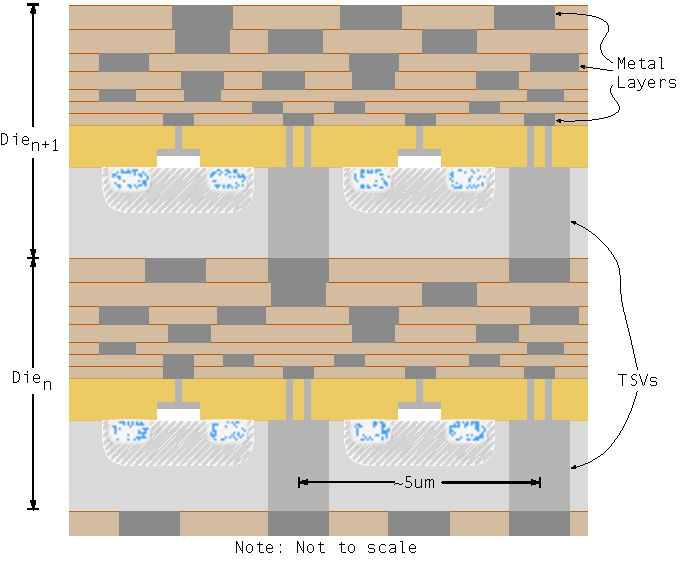
\includegraphics[width=4.5in]{TSVs.pdf}}
}
\caption{Die Stack profile \cite{itrs2015_interconn} with \acp{tsv}}
\label{fig:tsv}
\end{figure}

There are other definitions on how the dies are bonded together:
\begin{outline}
  \1 Wafer-to-Wafer
    \2 current \ac{esd} mitigation allows implementation of unbuffered IO
    \2 potential low yield because of lack of knowledge regarding \ac{kgd}
  \1 Die-to-Wafer
    \2 will need additional \ac{esd} mitigation support
    \2 higher yield because of knowledge of \ac{kgd}
  \1 Die-to-Die
    \2 will need additional \ac{esd} mitigation support
    \2 higher yield because of knowledge of \ac{kgd}
\end{outline}

This work is targeting \ac{3dic} technology that supports 3D-Stacked \ac{soc} or 3D-Stack \ac{ic} with high levels of interconnect.
To avoid using large IO buffers for the \ac{tsv} interconenct, this work assumes that the \ac{3dic} technology supports unbuffered interconnects. 
This would suggest wafer-to-wafer bonding because of the existing \ac{esd} mitigation during wafer handling although it is anticipated that improved \ac{esd} mitigation will be introduced in future manufacturing steps.

The technology roadmap in \cite{itrs2015_interconn} and the information in \cite{patti2014} suggests \SI{5}{\micro\meter} pitch \acp{tsv} is a reasonable design goal. This work assumes a one-to-one ration of signal \acp{tsv} to power/grod \ac{tsv} so when accounting for area associated with \acp{tsv}, the number of signal \acp{tsv} are doubled.

As a large amount of \acp{tsv} are employed, \ac{tsv} energy cannot be ignored.
Most of the energy dissipated in the \ac{tsv} is associated with the charging and discharging of the \acp{tsv} capacitance. For a \SI{5}{\micro\meter} pitch and \SI{2}{\micro\meter} radius \acp{tsv}, \cite{Bamberg2017} table I suggests an average capacitance of \SI{4.2}{\femto\farad} \footnote{\cite{tezzaron:preso} suggests a lower capacitance}.

Based on \eqref{eq:Energy in a Capacitor} and assuming a supply voltage of \SI{1.0}{\volt}, the power associated with a \ac{tsv} is shown in equation \eqref{eq:Energy in a TSV}.

\begin{alignat}{2} 
\label{eq:Energy in a Capacitor}
\text{Energy to charge a \ac{tsv},\hspace{4mm}} E_{tsv} &= \frac{1}{2} \cdot C_{tsv} \cdot V^2  %\SI{}{\joule} \\
\end{alignat}

\begin{alignat}{2} 
\label{eq:Energy in a TSV}
\text{Energy to charge a \ac{tsv},\hspace{4mm}} E_{tsv} &= \frac{1}{2} \cdot C_{tsv} \cdot V^2  = \frac{1}{2} \cdot \num{4.2e-15} \cdot 1.0 = \SI[per-mode=symbol]{2.1}{\femto \joule} \nonumber \\
\text{Power per \ac{tsv},\hspace{4mm} } P_{tsv} &= E_{tsv} \cdot \text{bit rate} \nonumber \\
\text{normalizing to a clock of \SI{1.0}{\giga\hertz}} & \nonumber \\
\text{Power per \ac{tsv} per \SI{}{\hertz} } &= \SI[per-mode=symbol]{2.1}{\micro \watt \per \giga \bit\per\second \per \ac{tsv}}
\end{alignat}

The \ac{tsv} design guidelines used by this work are summarized in table \ref{tab:TSV Design Characteristics}.
%Therefore, this work assumes \acp{tsv} with a \SI{5}{\micro\meter} pitch and a power dissipation of \SI[per-mode=symbol]{2.1}{\micro \watt \per \giga \bit\per\second \per \ac{tsv}}.

\begin{table}[h*]
  \captionsetup{justification=centering, skip=3pt}
  \caption{TSV Design Characteristics}
  \vspace{3pt}
  \label{tab:TSV Design Characteristics}
  \centering
    \begin{adjustbox}{width=0.6\textwidth}
      \begin{tabular}{cccc}
        \toprule
                                         &      \multicolumn{2}{c}{Dimensions}       &                                                                                  \\  %\cline{1-1}
                   Parameter             &        Pitch        &    Radius           &  Power                                                                          \\
        \hline  % instead of \midrule %midrule doesnt ove        
                   Value                 &\SI{5}{\micro\meter} &\SI{2}{\micro\meter} &\SI[per-mode=symbol]{2.1}{\micro \watt \per \giga \bit\per\second \per \ac{tsv}}\cite{Bamberg2017}  \\
        \bottomrule
      \end{tabular}
    \end{adjustbox}
    \vspace{3pt}
\end{table}







%% Lee
%% In dissertation, change 
%    section* to chapter 
%    subsection* to section
%    subsubsection* to subsection

% >>>>>>>>>>>>>>>>>>>>>>>>>>>>>>>>>>>>>>>>>>>>>>>>>>>>>>>>>>>>>>>>>>>>>>>>>>>>> DRAM Customizable <<<<<<<<<>>>>>>>>>>>>>>>>>>>>>>>>>>>>>>>>>>>>>>>>>>>>>>>>>><<<<<<<<<<<<<
\chapter{DRAM Customizations}
\label{sec:DRAM Customizations}

There are two types of memory employed in \acp{asic} and \acp{asip}, \acl{sram} or \ac{sram} and \acl{dram}, or \ac{dram}.
Both of these technologies have a similar top level block diagram which contains an array of storage elements, a means to address into a particular row of memory cells and a means to read and write a column of those cells.
A basic block diagram is shown in figure \ref{fig:MemoryBlockDiagram}.
\begin{figure}[!t]
% the [] contains position info e.g. [!t] means here
\centering
\captionsetup{justification=centering}
\centerline{
\mbox{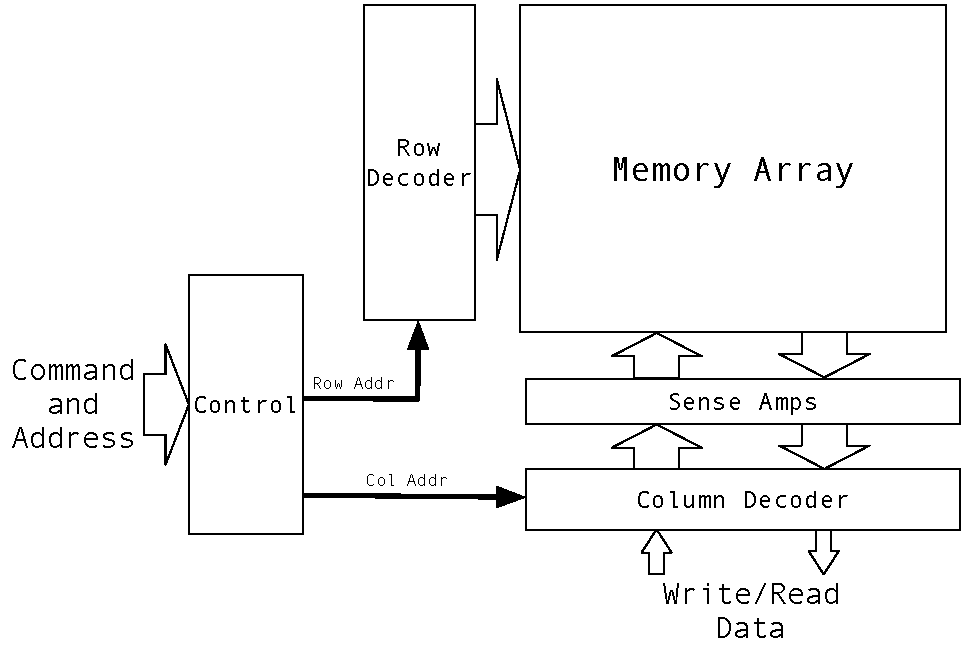
\includegraphics[width=.8\linewidth]{BasicMemoryBlockDiagram}}
}
\caption{Typical Memory Block Diagram \cite{Jacob:2007:MSC:1543376}}
\label{fig:MemoryBlockDiagram}
\end{figure}


\begin{figure}
\centering
\begin{subfigure}{.45\textwidth}
  \centering
  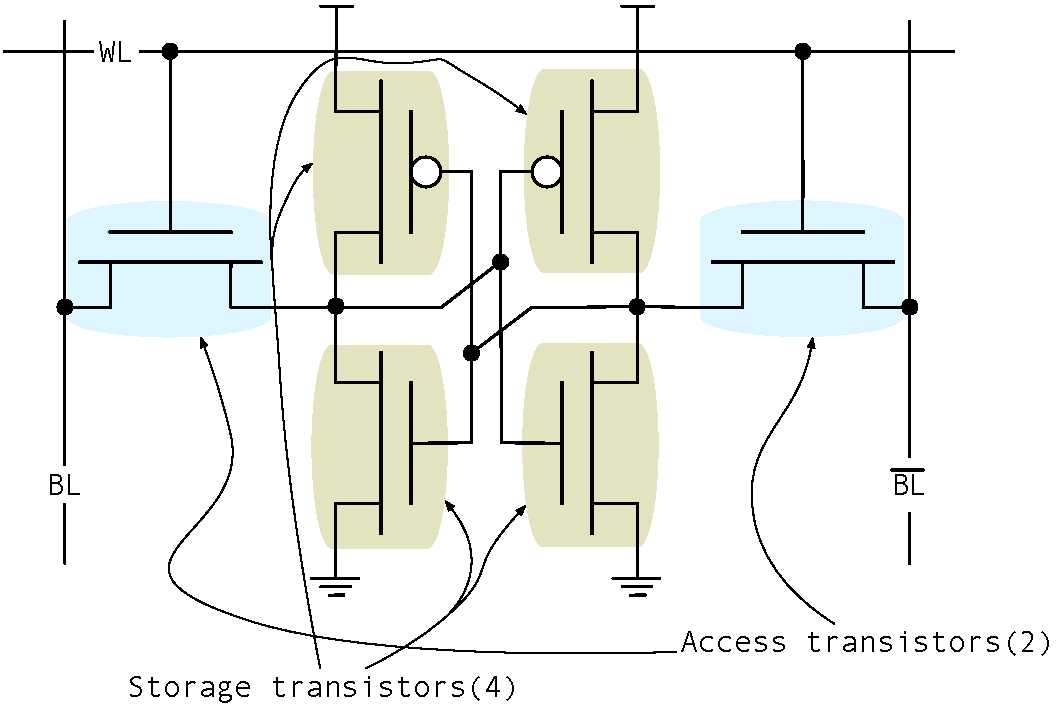
\includegraphics[scale=0.4]{SRAM_Cell}
  \captionsetup{justification=centering, skip=5pt}
  \vspace{-6pt}
  \caption{SRAM Storage Cell \cite{Jacob:2007:MSC:1543376}}
  \label{fig:SRAM Cell}
\end{subfigure}%
\begin{subfigure}{.45\textwidth}
  \centering
  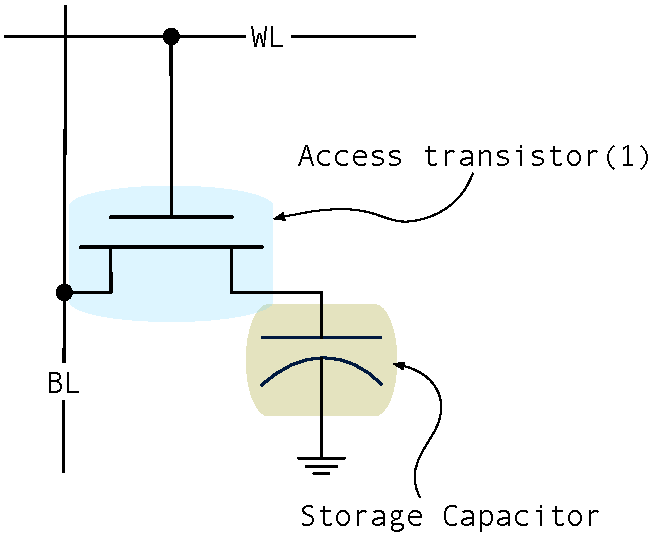
\includegraphics[scale=0.4]{DRAM_Cell}
  \captionsetup{justification=centering, skip=5pt}
  %\vspace{36pt}
  \vspace{20pt}
  \caption{DRAM Storage Cell \cite{Jacob:2007:MSC:1543376}}
  \label{fig:DRAM Cell}
\end{subfigure}
\captionsetup{justification=centering, skip=12pt}
\caption{RAM Storage Cell Types}
\label{fig:Memory Storage Cells}
\end{figure}


Accessing a typical \ac{sram} involves providing an address and either reading or writing the contents of that location. 
The read or write often completes in one or two clock cycles depending on whether the \ac{sram} employs internal registers which are used run the \ac{sram} with a faster clock.

The storage cell inside the \ac{sram} is formed from cross-coupled transisters (see figure \ref{fig:SRAM Cell}) which latch the contents and hold the contents indefnitely or until power is removed from the device.
The storage structure employs six transistors and allows the access logic to be relatively simple and fast but has a relatively low XXXXXXXXXXXX capacity.

Accessing a "typical" DRAM is much more involved, it involves opening a page in a bank, reading or writing a portion of the contents of the page then closing the page. 

The reasons behind this added complexity is the memory cell inside the \ac{dram} which is formed from a capacitor (see figure \ref{fig:DRAM Cell}) which holds a charge reflecting a logic zero or one. 
The major difference between the \ac{sram} cell is the number of elements it takes to implement. The size of the \ac{dram} cell means \ac{dram} arrays provide five to six times more storage when compared to a similar sized \ac{sram} array.
The major disadvantage is the capacitor cannot hold a indefnitely because the leakage currents in \acp{ic} cause the charge to leak away. If kept unchecked, the stored value will dissipate and it is this behavior that makes accessing a \ac{dram} array more complicated than a similar \ac{sram} array.

When an \ac{sram} cell is read, the cross-coupled transistors retain the stored value. The issue with \acp{dram} is when a storage cell is read, the capacitor is discharged. In addition, sensing this discharging capacitor takes long time to sense when compared to the \ac{sram} cell.
To alleviate this problem, \ac{dram} arrays are formed from a column of storage elements known as a page. When the read occurs, the entire contents of the page are transferred to registers. Once this transfer is complete, portions of the page can be read similar to reading an \ac{sram}. 
The problem is that if another read wants to access data that is not in the page, the page has to be closed and another page opened. This involves transferring the previously registered page back to the array to recharge the capacitors in the pages storage elements. The next page can then be read and transferred to the page registers.
The process of opening and closing pages is a relatively long time, typically 10-20\SI[per-mode=symbol]{}{\nano\second}. So if the accesses are somewhat random, accesses are very slow when compared to \ac{sram}.
To get around this issue, the \ac{dram} is formed from more than one array of storage elements, between 8 and 32, know as banks. The idea is that while a page from one bank is being accessed, another bank can be opened in preparation for a future read (or write).
This access protocol is rather complicated and if consequtive accesses are not sequenced carefully, the performance of \ac{dram} can be poor.

The sequence of accesses cannot always be controlled, especially in general purpose computers, so \ac{sram} is typically used as the first level of memory with \ac{dram} used as the primary storage. 
using \ac{sram} as this first level memory is called a cache and these have been used for decades to isolate the computing system from unpredictable access behavior of the \ac{dram}.

As mentioned in section \ref{sec:overview} much of the \ac{asic} and \ac{asip} \ac{ann} research has focused on taking advantage of the performance and ease of use of \ac{sram}, but with this works target application an \ac{asic} or \ac{asip} employing \ac{sram} as its primary memory cannot be implemented with adequate storage capacity.
Under these circustances, \ac{dram} bandwidth will be the bottleneck.

This work focuses on using \ac{dram} as the primary storage and managing the accesses to ensure the \ac{dram} is used effectively. 
With the additional \ac{dram} customizations discussed in section \ref{sec:Very-Wide Bus} and \ref{sec:Write Mask}, this work demonstrates \ac{dram} bandwidths 10X faster than what is available with 2 or 2.5D solutions.
This high level of \ac{dram} bandwidth provides this work the ability to process multiple disparate \acp{ann} at or near real-time whilst being \textbf{\textcolor{black}{10-100X faster than state-of-the-art solutions}}.


\section{Customization One: Very-Wide Bus}
\label{sec:Very-Wide Bus}

Typically a bank may contain of the order of a few thousand pages and a page may contain of the order of a few thousand bits.

Once the page is open, the user accesses a portion of the requested page over a bus. With PCB based DRAMs the bus might vary from four to 16 bits wide, but with 3D DRAMs, such as HBM the bus might be up to 128 bits wide.

Figure \ref{fig:dramBlockDiagram} shows a block diagram of a typical DRAM.

\begin{figure}[!t]
% the [] contains position info e.g. [!t] means here
\centering
\captionsetup{justification=centering}
\centerline{
\mbox{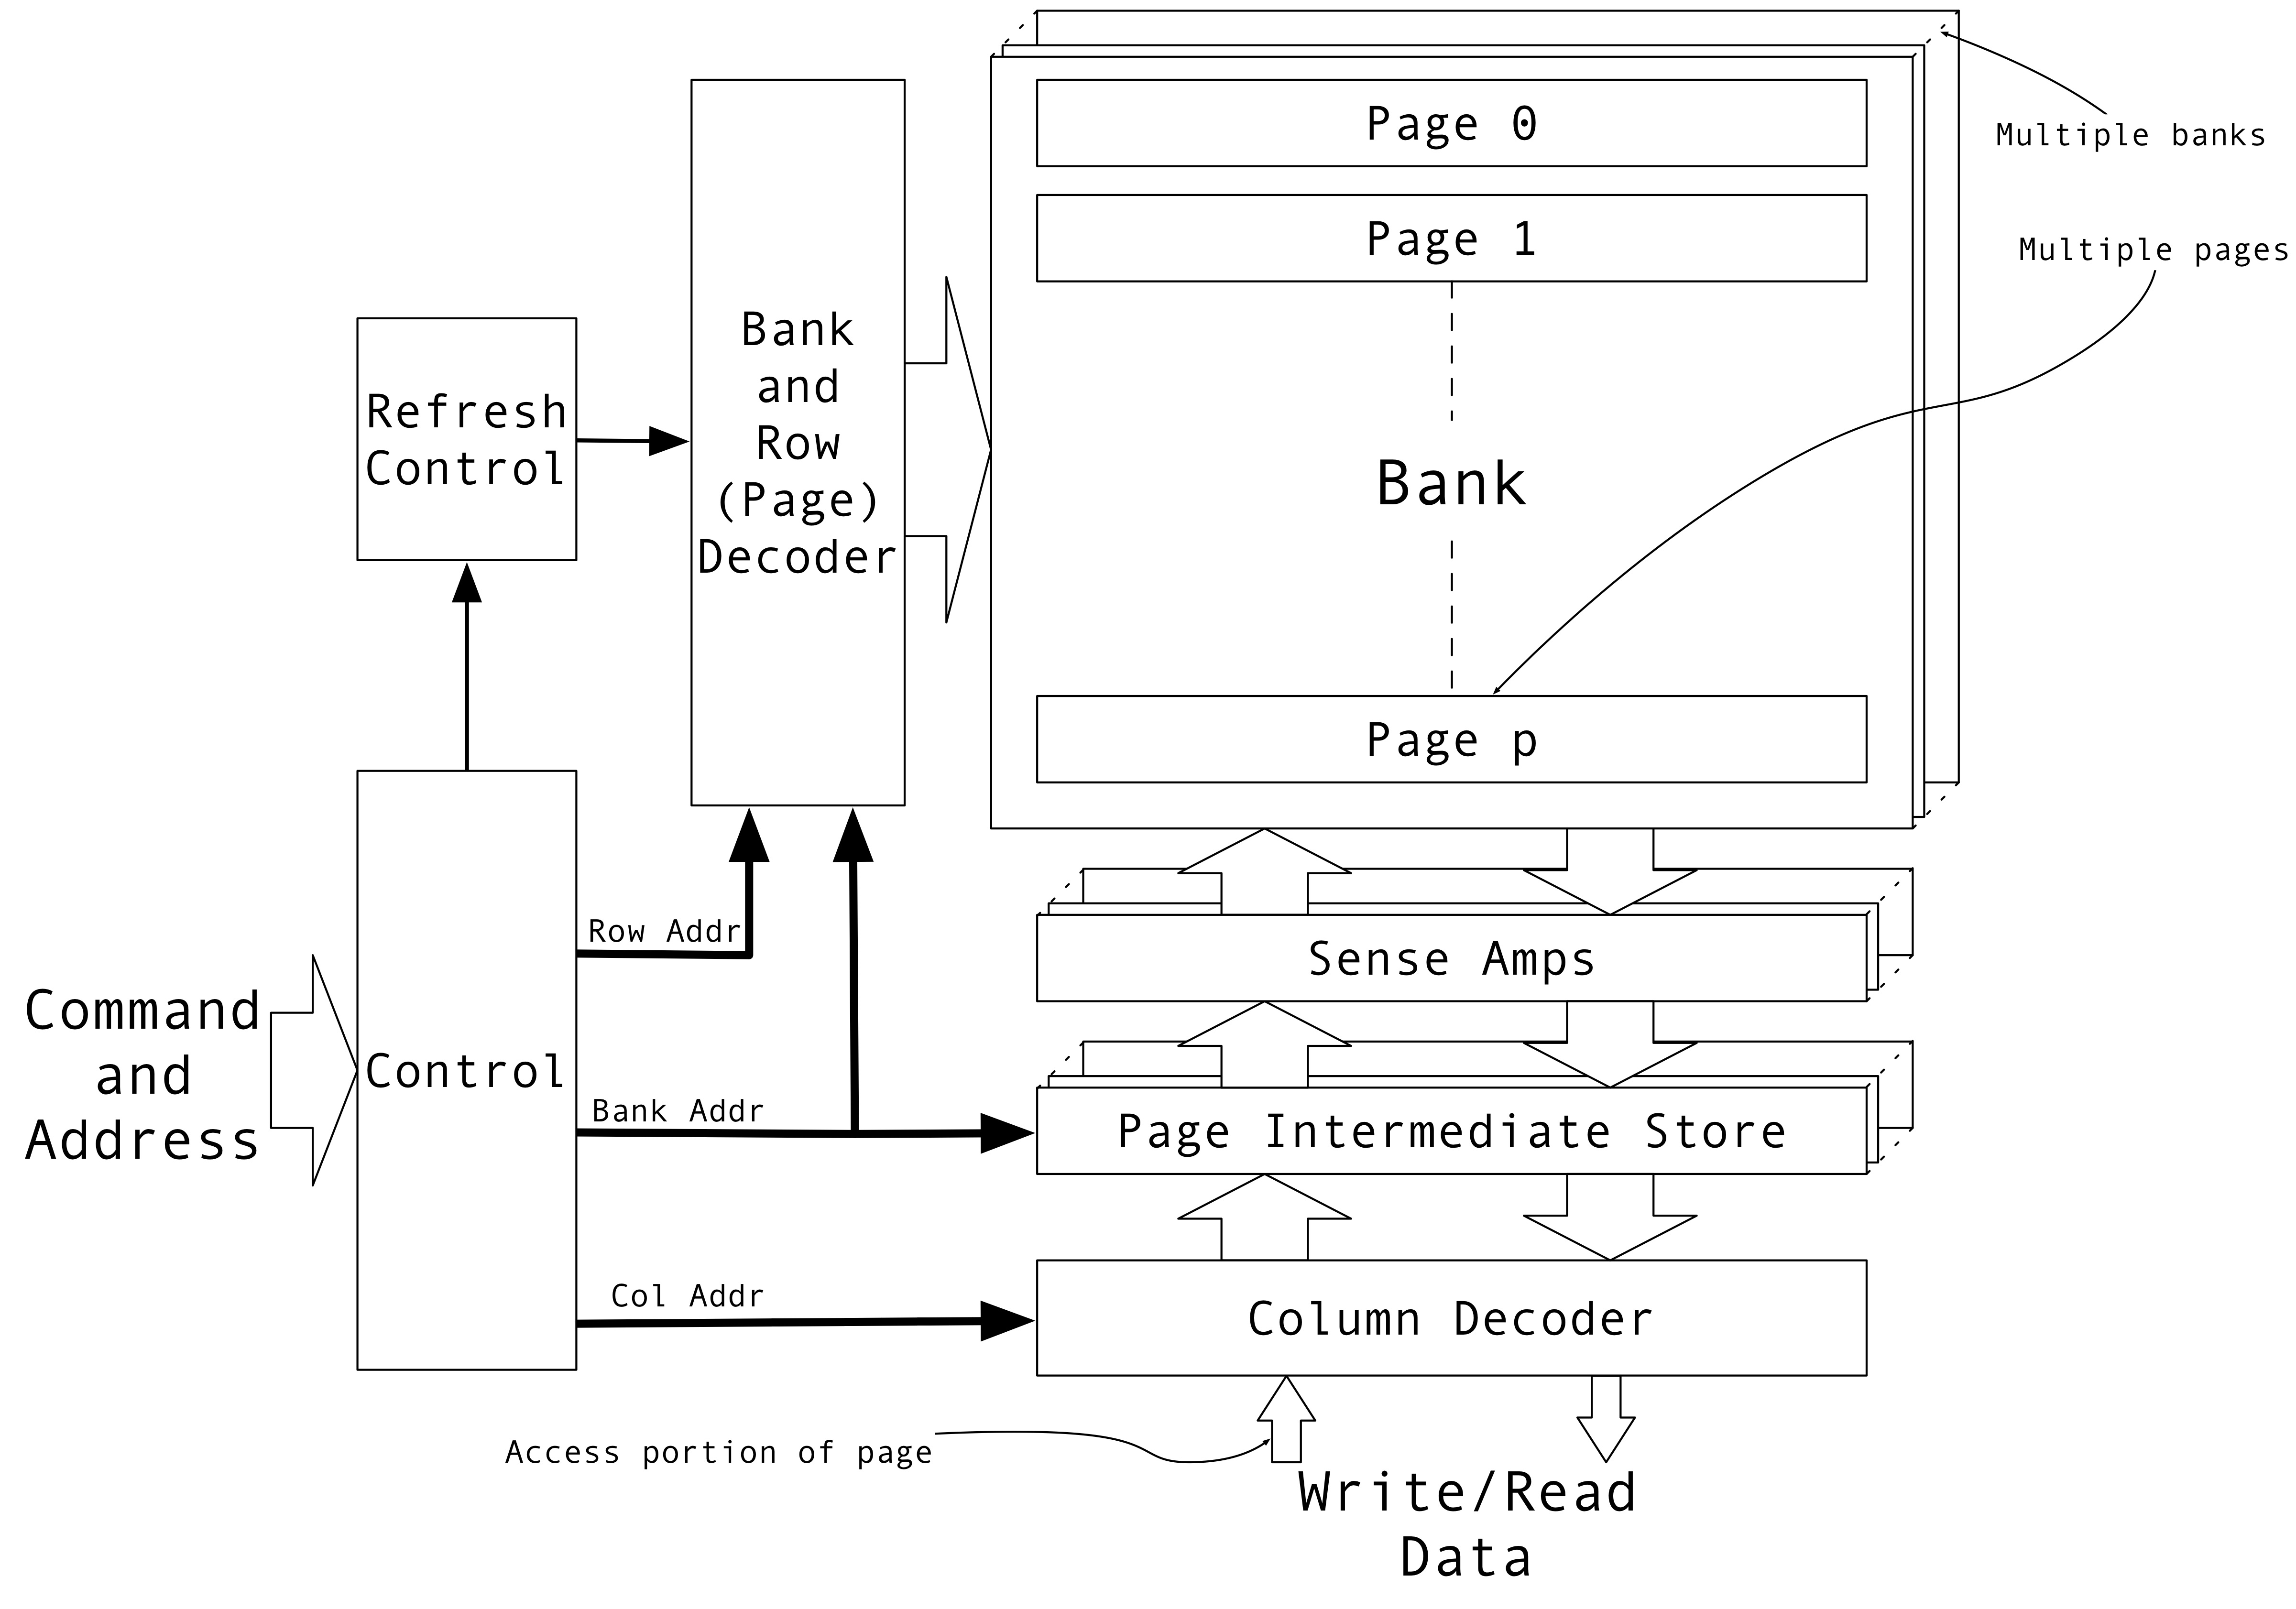
\includegraphics[width=.75\linewidth]{DRAMBlockDiagram.jpg}}
}
\caption{Typical DRAM Block Diagram}
\label{fig:dramBlockDiagram}
\end{figure}

This work achieves the increase in bandwidth by proposing that the DRAM expose more of its currently open page.

Without the limitations of having to transfer data beyond the chip stack, this work suggests exposing a larger portion of the page over a very wide bus. By staying within the 3D footprint, this bus can be implemented using fine pitch through-silicon-vias.
(see figure \ref{fig:dramBusChange}).

\begin{figure}[!t]
% the [] contains position info e.g. [!t] means here
\centering
\captionsetup{justification=centering}
\captionsetup{width=.75\linewidth}
\centerline{
\mbox{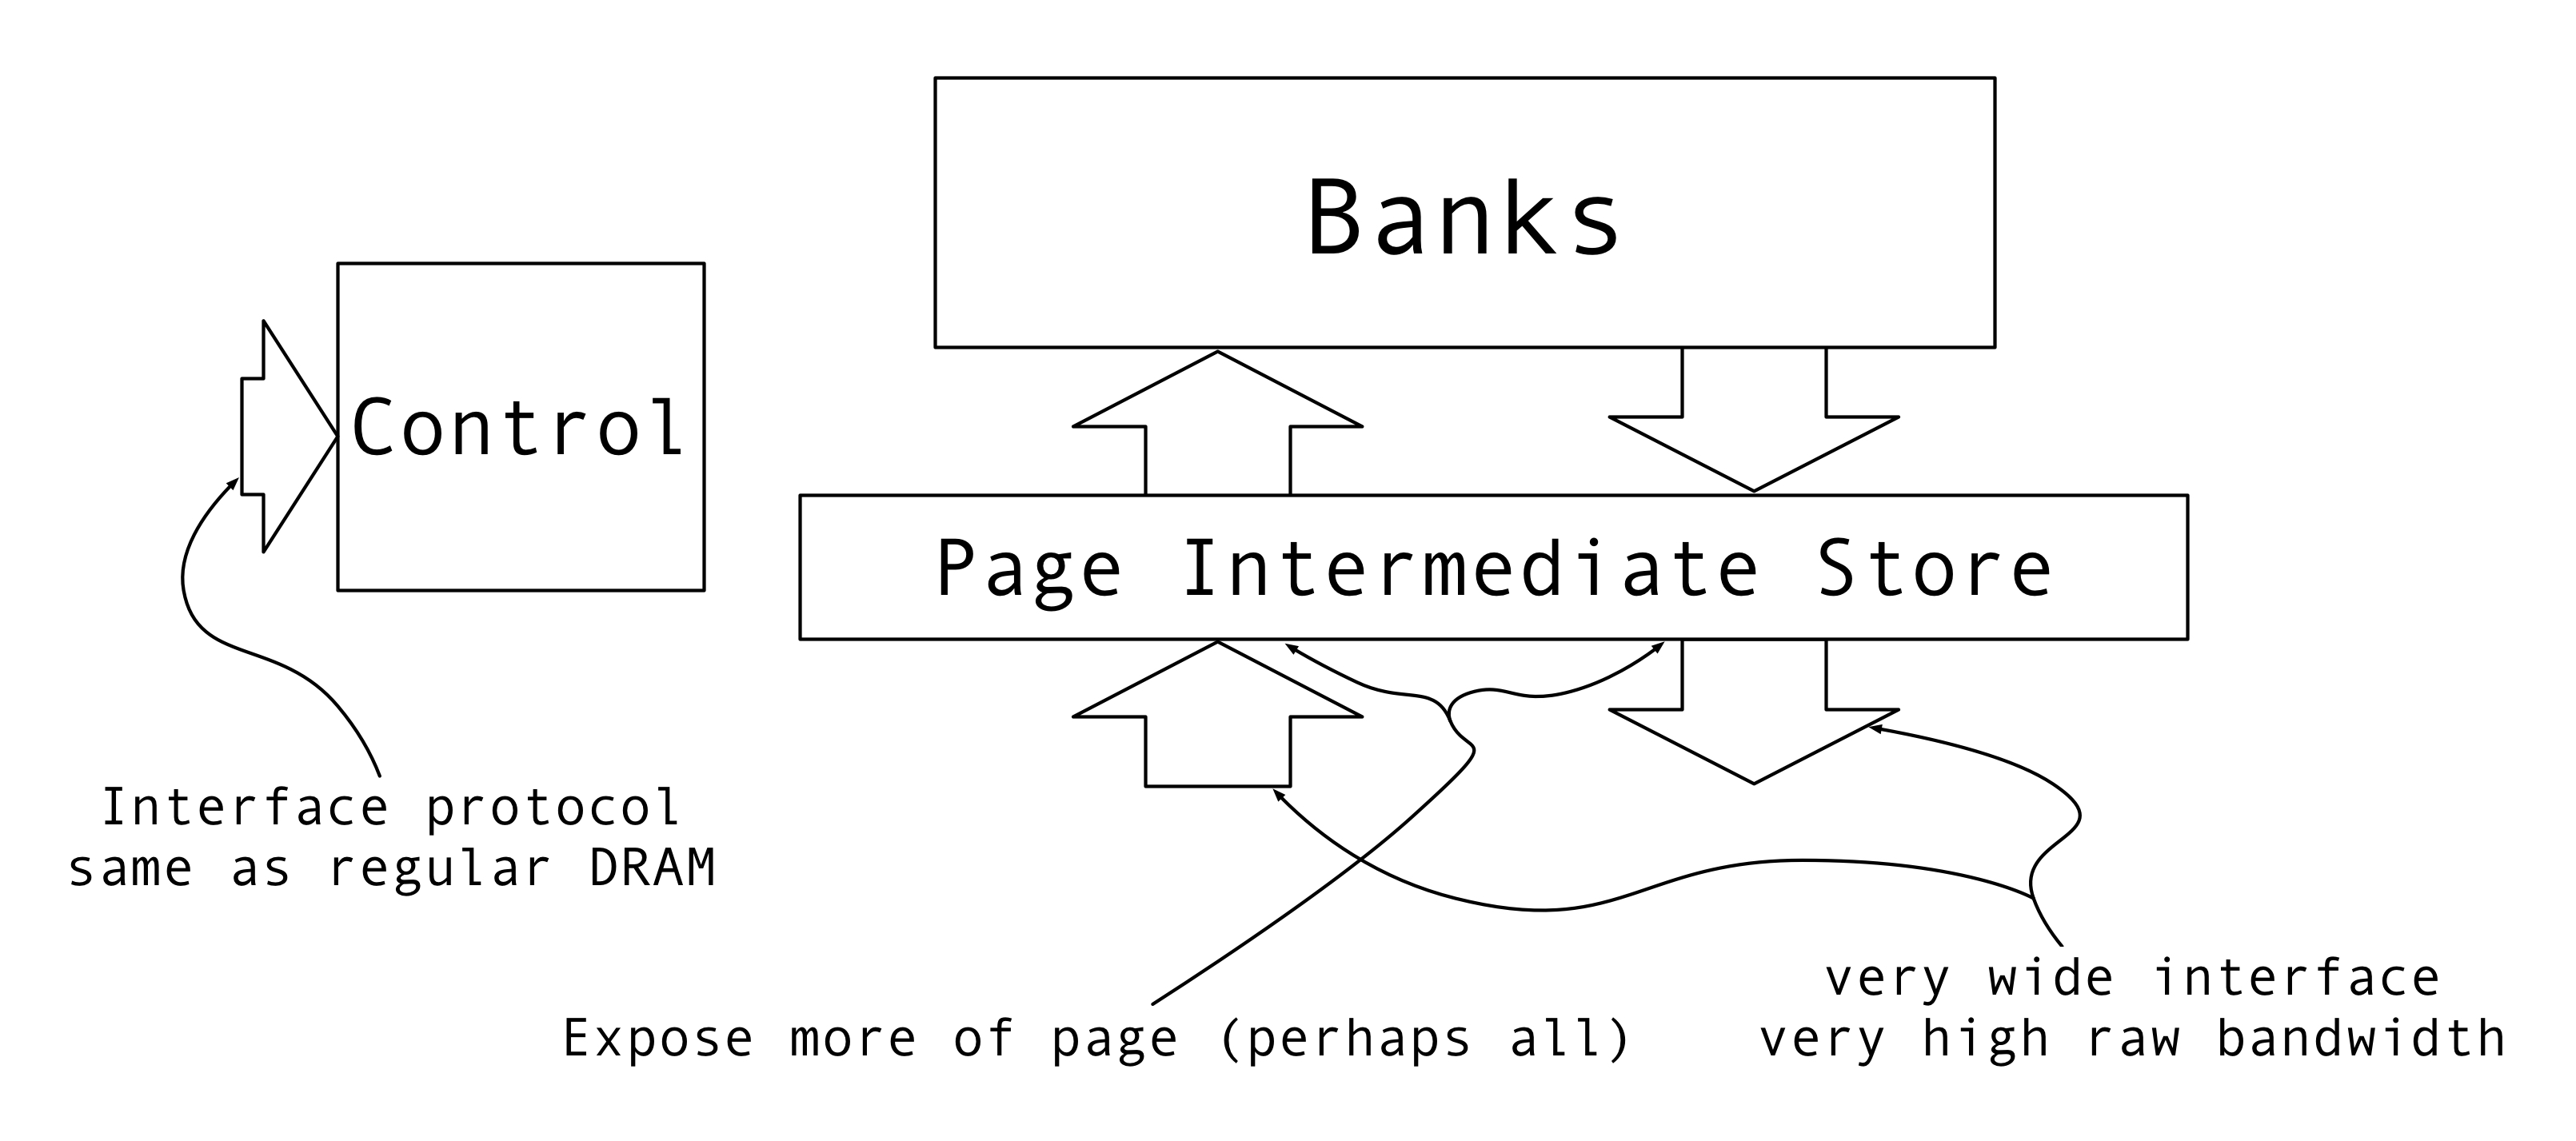
\includegraphics[width=.9\linewidth]{DRAMBusChange.jpg}}
}
\caption{Exposing more of the DRAM page}
\label{fig:dramBusChange}
\end{figure}

This work assumes the \ac{dram} interface protocol uses \ac{ddr} with a bus width of 2048. Given the \ac{diram4} employs a burst of two for read and write cycles, an entire \ac{diram4} page of 4096-bits is accessed during each read or write. 

\section{Customization Two: Write Mask}
\label{sec:Write Mask}
When processing an ANN, to compute the activation of an individual AN involves reading the pre-synaptic AN activations and the weights of the connections between the pre-synaptic ANs and the AN being processed. The activation of the processed AN is written back to memory. The ratio of reads to writes is high, 100s or 1000s to one. Therefore, the system often needs to write a portion of the page back to memory. To avoid a read/modify/write, a customization to the DRAM is the addition of a write data mask to the DRAM write path.

This work assumes single precision floating point for \ac{ann} weights and activation, so a mask bit will be provided on a word basis or every 32-bits.


%% Lee
%% In dissertation, change 
%    section* to chapter 
%    subsection* to section
%    subsubsection* to subsection

% >>>>>>>>>>>>>>>>>>>>>>>>>>>>>>>>>>>>>>>>>>>>>>>>>>>>>>>>>>>>>>>>>>>>>>>>>>>>> DRAM Customizable <<<<<<<<<>>>>>>>>>>>>>>>>>>>>>>>>>>>>>>>>>>>>>>>>>>>>>>>>>><<<<<<<<<<<<<
\chapter{DRAM Customizations}
\label{sec:DRAM Customizations}

Accessing a "typical" DRAM involves opening a page in a bank, reading or writing a portion of the contents of the page then closing the page.

Typically a bank may contain of the order of a few thousand pages and a page may contain of the order of a few thousand bits.

Once the page is open, the user accesses a portion of the requested page over a bus. With PCB based DRAMs the bus might vary from four to 16 bits wide, but with 3D DRAMs, such as HBM the bus might be up to 128 bits wide.

Figure \ref{fig:dramBlockDiagram} shows a block diagram of a typical DRAM.

\begin{figure}[!t]
% the [] contains position info e.g. [!t] means here
\centering
\captionsetup{justification=centering}
\centerline{
\mbox{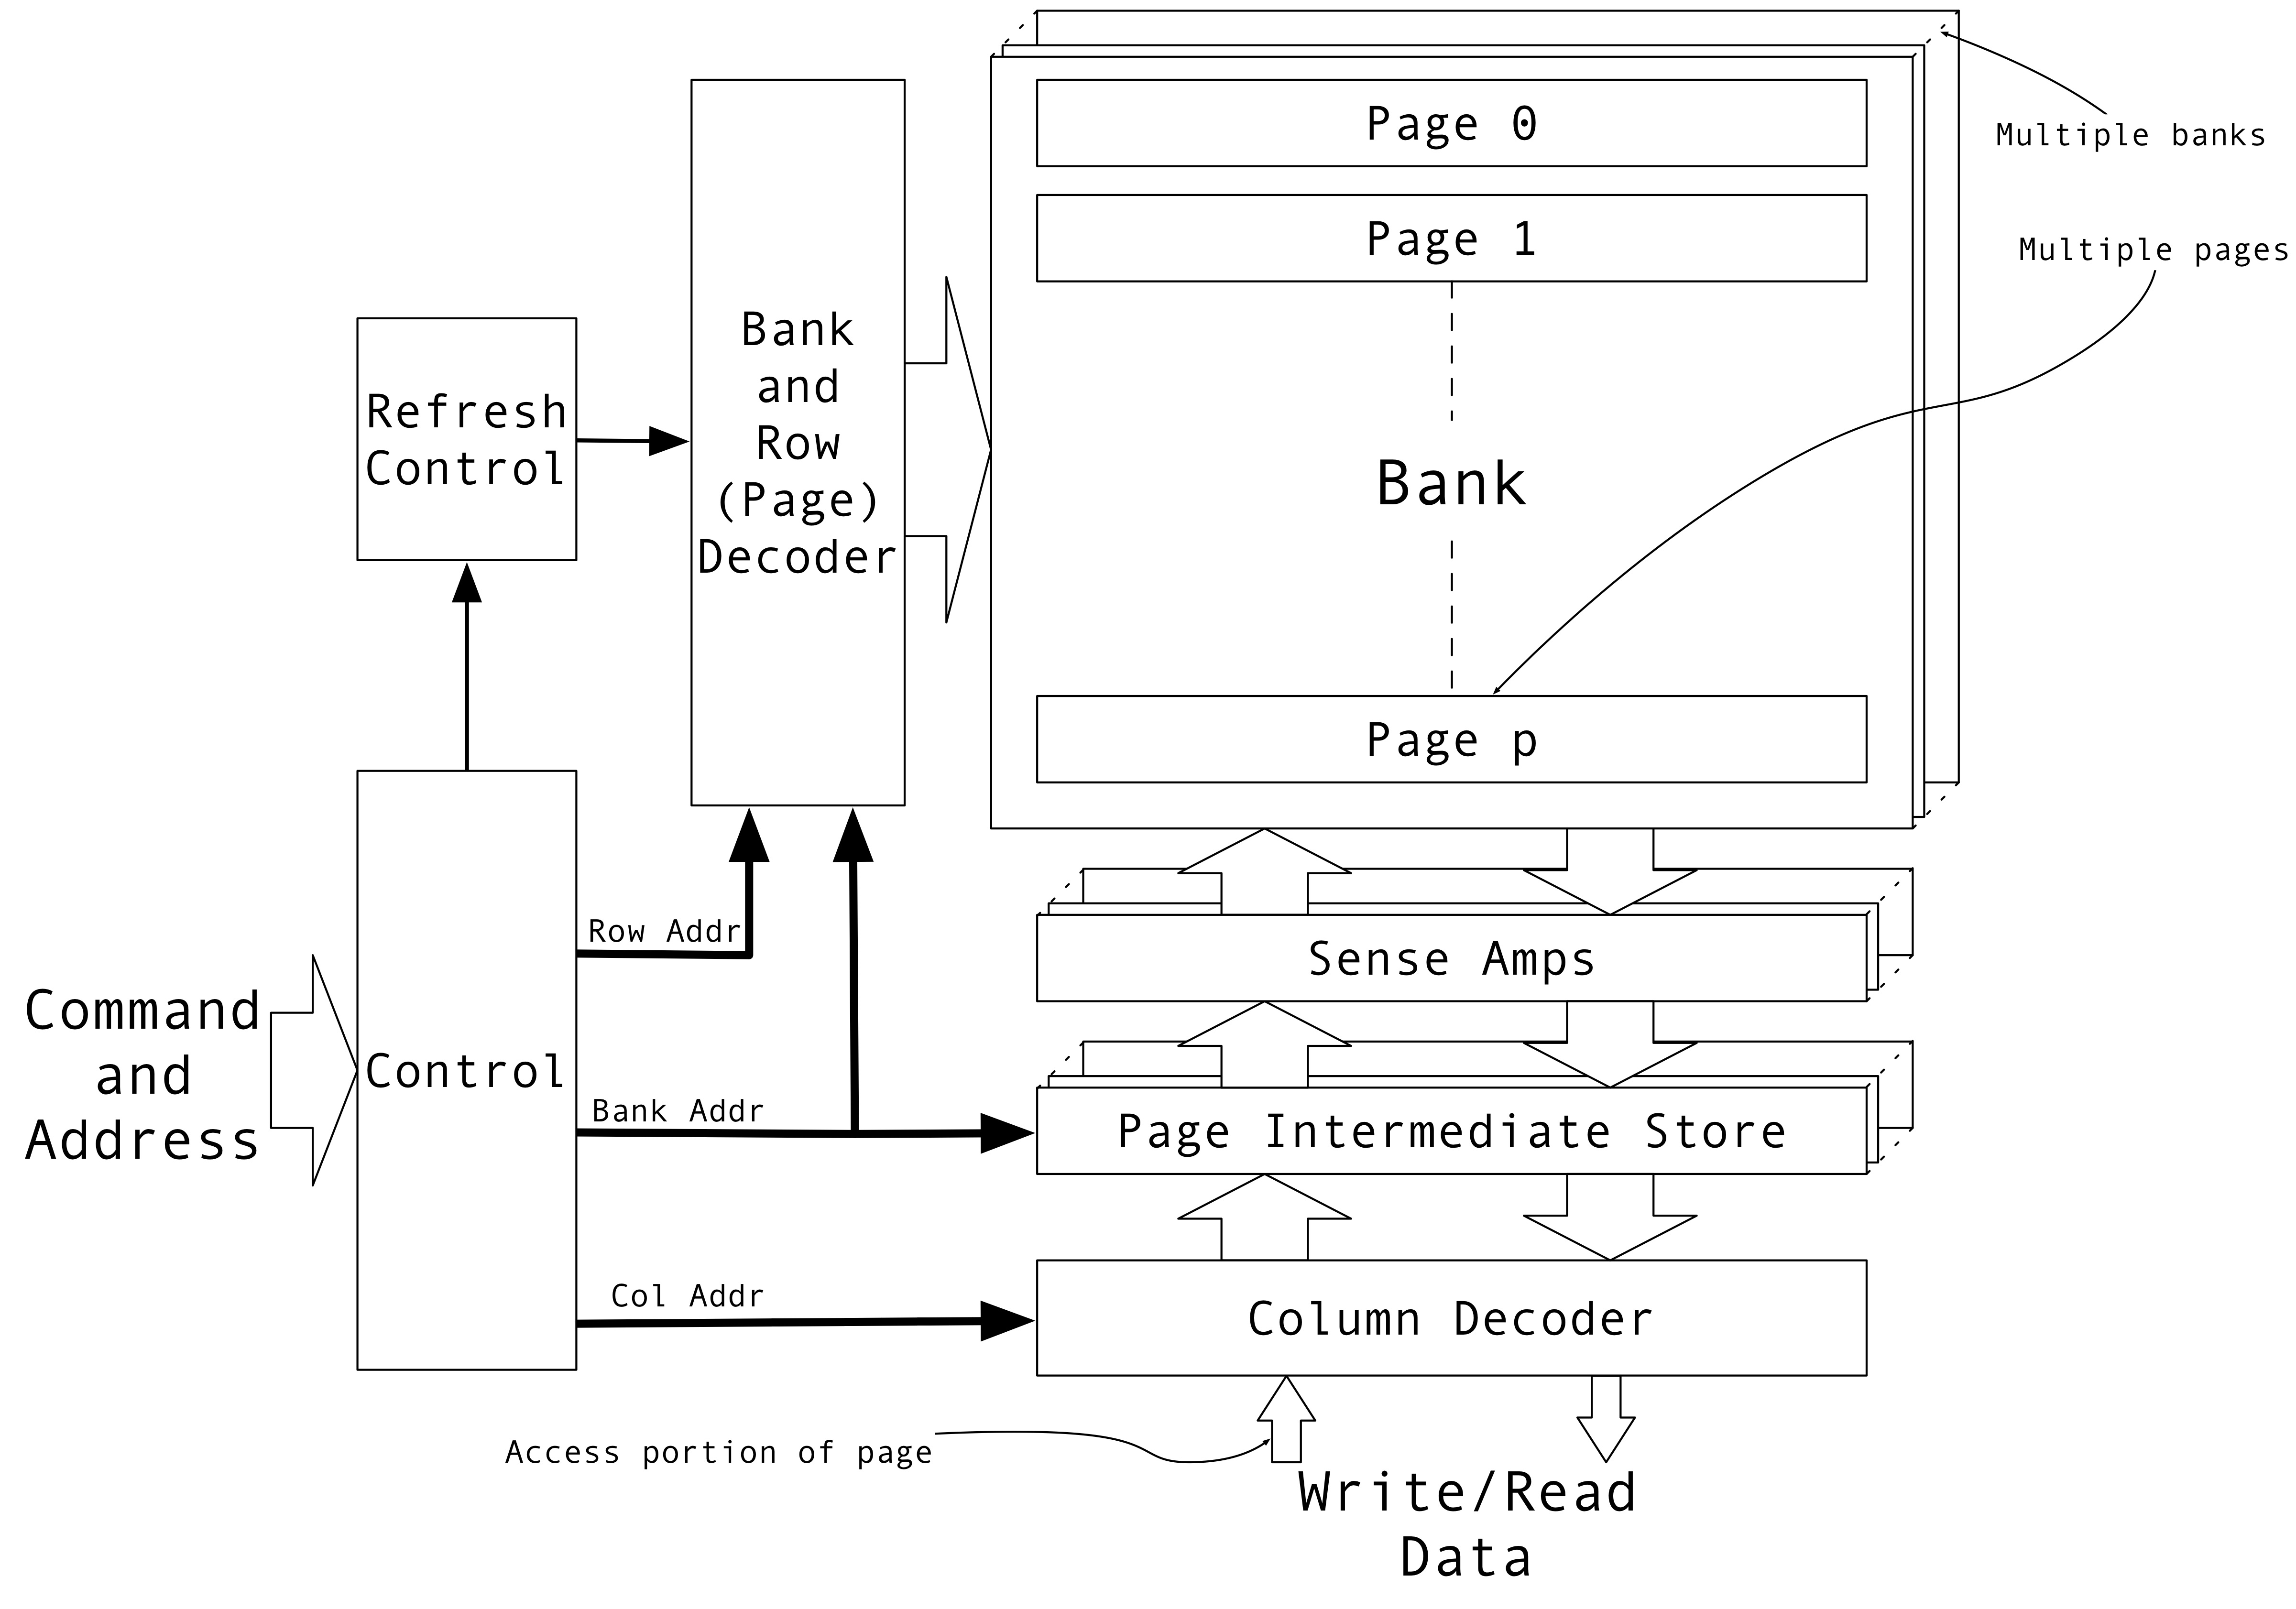
\includegraphics[width=.9\linewidth]{DRAMBlockDiagram.jpg}}
}
\caption{Typical DRAM Block Diagram}
\label{fig:dramBlockDiagram}
\end{figure}

\section{Very-Wide Bus}
\label{sec:Very-Wide Bus}

This work achieves the increase in bandwidth by proposing that the DRAM expose more of its currently open page.

Without the limitations of having to transfer data beyond the chip stack, this work suggests exposing a larger portion of the page over a very wide bus. By staying within the 3D footprint, this bus can be implemented using fine pitch through-silicon-vias.
(see figure \ref{fig:dramBusChange}).

\begin{figure}[!t]
% the [] contains position info e.g. [!t] means here
\centering
\captionsetup{justification=centering}
\captionsetup{width=.9\linewidth}
\centerline{
\mbox{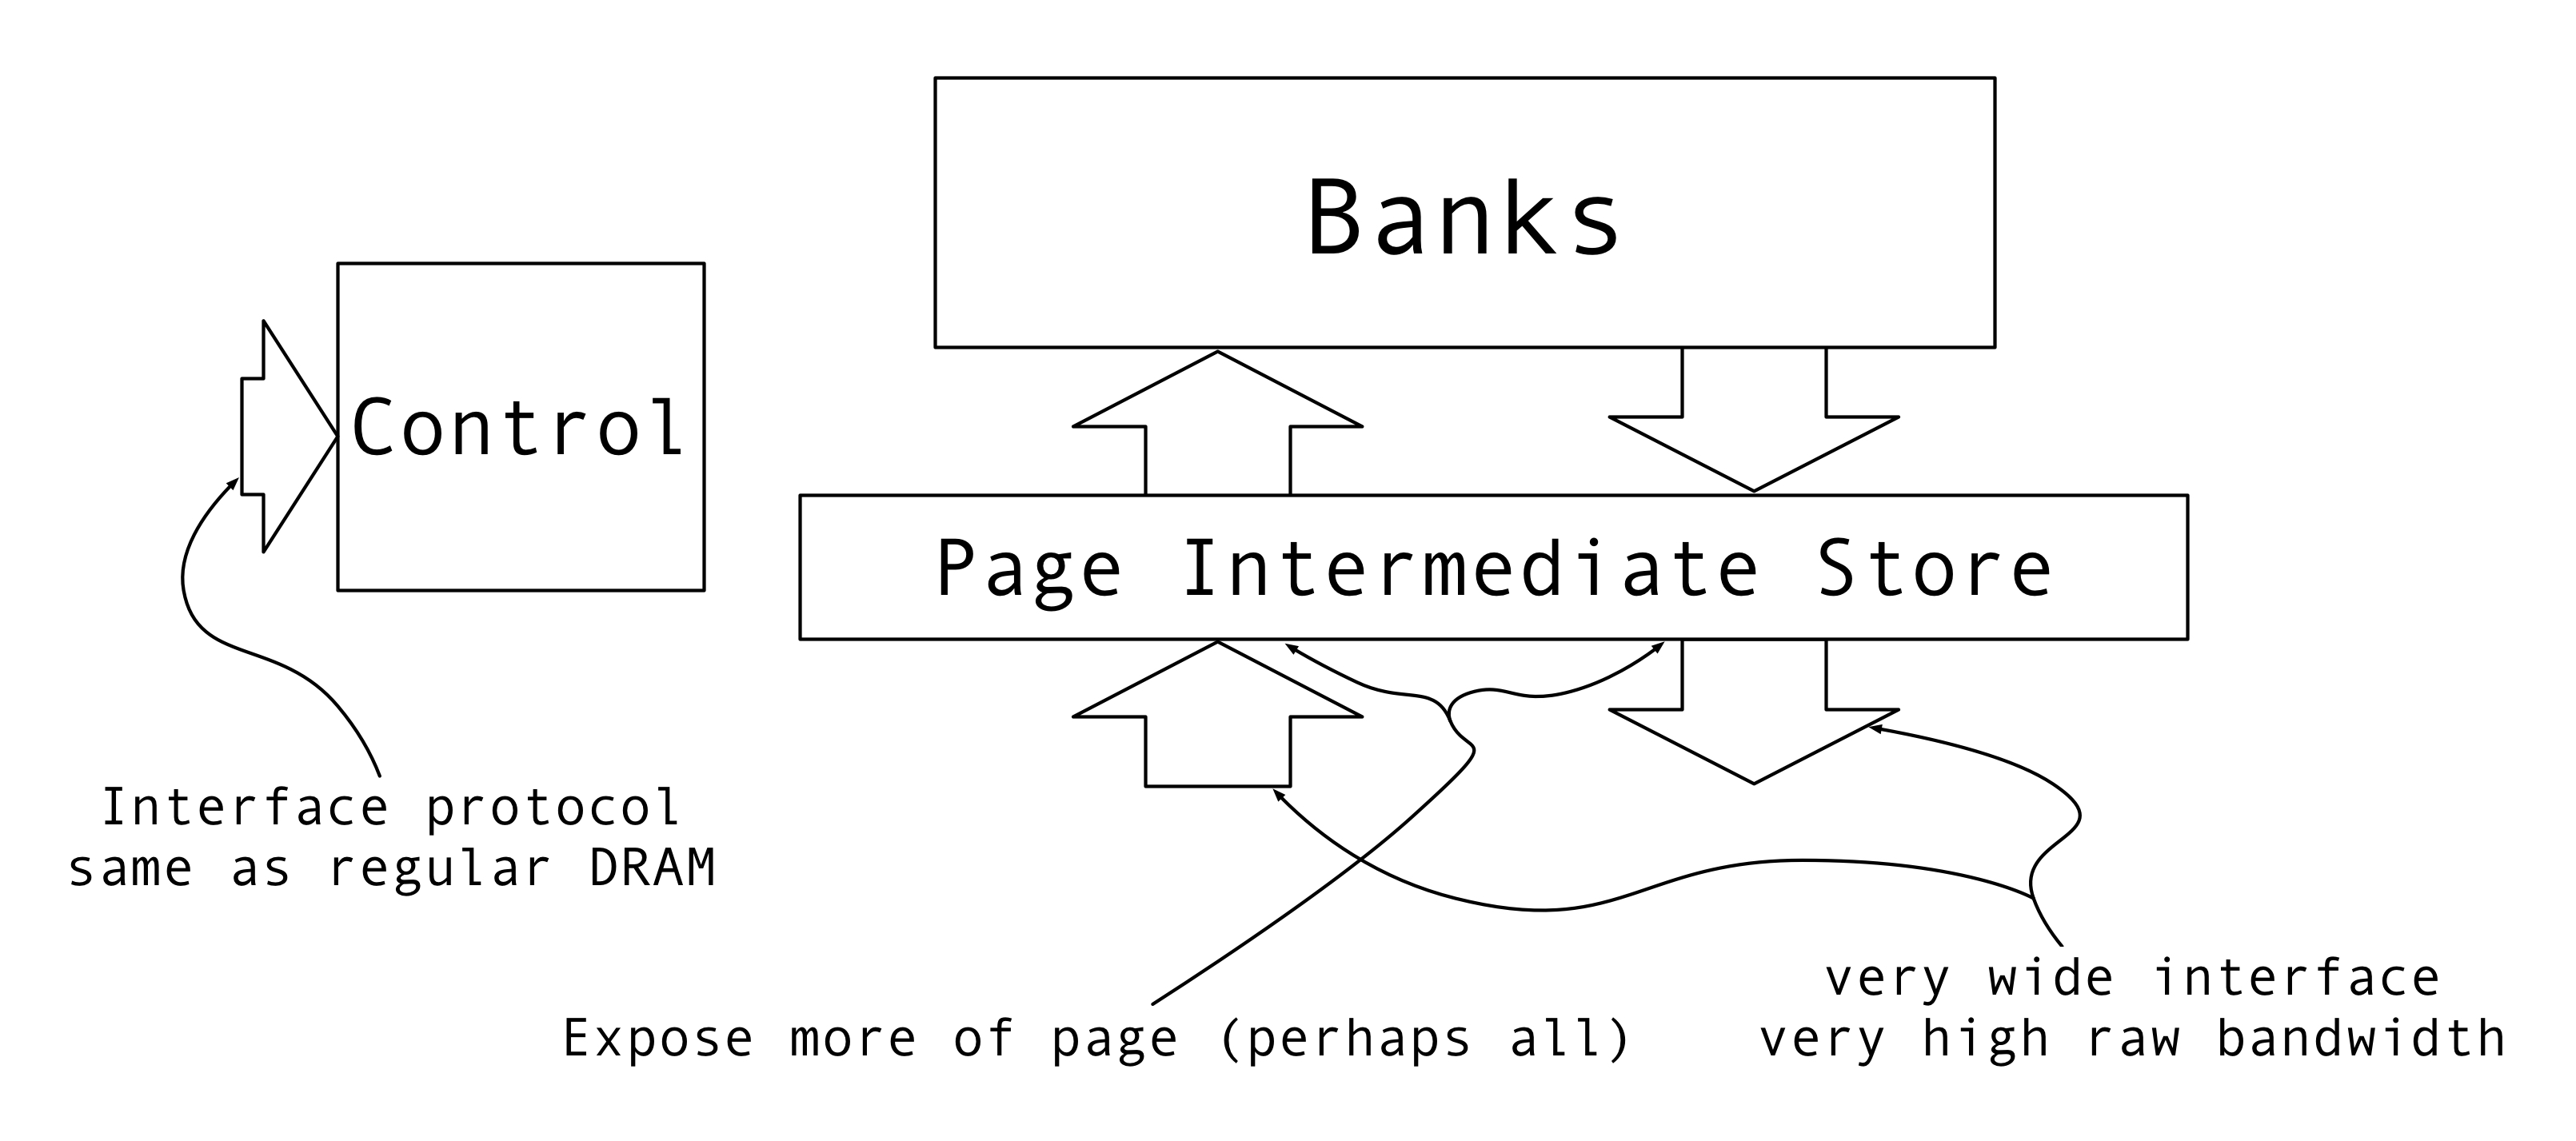
\includegraphics[width=.9\linewidth]{DRAMBusChange.jpg}}
}
\caption{Exposing more of the DRAM page}
\label{fig:dramBusChange}
\end{figure}

\section{Write Mask}
\label{sec:Write Mask}
When processing an ANN, to compute the activation of an individual AN involves reading the pre-synaptic AN activation's and the weights of the connections between the pre-synaptic ANs and the AN being processed. The activation of the processed AN is written back to memory. The ratio of reads to writes is high, 100's or 1000's to one. Therefore, the system often needs to write a portion of the page back to memory. To avoid a read/modify/write, a customization to the DRAM is the addition of a write data mask to the DRAM write path.


%% Lee
%% In dissertation, change 
%    section* to chapter 
%    subsection* to section
%    subsubsection* to subsection


% #######################################################################################################################################
%\chapter{Detailed System Description}
%\label{chap-six}

%\restoregeometry


%%---------------------------------------------------------------------------%%
%%  Bibliography 

%%  You can use the bibitem list.
%\bibliographystyle{unsrt}
%\begin{%thebibliography}{99}
%\bibitem{cb02}
%Casella, G. and Berger, R.L. (2002)
%\newblock {\it Statistical Inference, Second Edition.}
%Duxbury Press, Belmont, CA.
%
%\bibitem{t06}
%Tsiatis, A.A. (2006)
%\newblock {\it Semiparametric Theory and Missing Data.}
%Springer, New York.
%
%\end{thebibliography}

%% or use BibTeX
%\bibliography{Ortiz-thesis}{}
%\bibliographystyle{plain}
%\nociterec{*}

%\bibliographystyle{plainnat}%plainnat is necessary to enable the use of citet. Natbib style file.
%\bibliography{Ortiz-thesis2}
%\ensureoddstart
\begin{spacing}{1}
 \setlength\bibitemsep{11pt} %22pt = 2*11pt, where fontsize is 11pt
 \phantomsection
 \addcontentsline{toc}{chapter}{{\uppercase{\bibname}}} %\textorpdfstring and \uppercase needed due to hyperref package http://www.latex-community.org/forum/viewtopic.php?f=44&t=16601
 %\vspace{-0.5in}
\titleformat{\chapter}[display]{\bf\filcenter
}{\chaptertitlename\ \thechapter}{11pt}{\bf\filcenter}
\titlespacing*{\chapter}{0pt}{-0.5in-9pt}{22pt}

\printbibliography[heading=myheading]
\end{spacing}
%\bibliographystyle{apalike}


%%---------------------------------------------------------------------------%%
% Appendices
%\ensureoddstart
\restoregeometry
\appendix
\newgeometry{margin=1in,lmargin=1.25in,footskip=\chapterfootskip, includehead, includefoot}



% #######################################################################################################################################
\chapter{Softmax Implementation}
\label{sec:Appendix-A}
\label{sec:Softmax Implementation}

In classifiers, the last layer is often implemented using a softmax \cite{wikipedia_softmax}\cite{stanford_softmax} function.
The outputs of this layer represent probabilties of each class/output.
As seen in Figure \ref{fig:classifier layer}, the classifier \ac{an} state calculation involves a \ac{mac} of the pre-synaptic \ac{an} states followed by an exponent.
The final \ac{an} state is the exponent of individual \acp{an} divided by the sum of all \acp{an} exponent value.

This work calculates the classifier \ac{an} states by separating the classifier into multiple layers as shown in Figure \ref{fig:classifier additional layers}.
The single classifier layer is implemented using three layers.
The first layer determines the exponent of each \ac{an}. This is accomplished using the \ac{stop} \ac{mac} operation followed by the \ac{simd} \ac{relu} and exponent \acp{sfu}.
The \ac{an} states of this layer are sent back to main memory.
The next layer is a single \ac{an} calculation, as described in Section \ref{sec:Processing a single ANe} with the pre-synatic weights set to unity.
The resulting calculation is an accumulation of the \ac{an} exponent values.
The \ac{simd} divider \ac{sfu} is then used to perform a reciprocal and the result is placed in a \ac{simd} register.
The final layer is calculated using the \ac{stop} to perform a multiplication of each presynaptic \ac{an} state with the reciprocal value held in the \ac{simd} register effectively performing the division in the softmax function.

Performing the Softmax funcion is relatively inefficient, however the time taken is masked by the time taken to perform the initial classifier layer \ac{an} state calculation.
An example calculation sequeuce is shown in Figure \ref{fig:classifier implementation sequence timing} using the baseline \ac{ann} which employs one thousand classifiers with four thousand presynapic \acp{an}.


\begin{figure}[h]
  \centering
  \captionsetup{justification=centering}
  \captionsetup{width=0.9\textwidth}
  \begin{minipage}{1\textwidth}
    \centering
    \centerline{
    \mbox{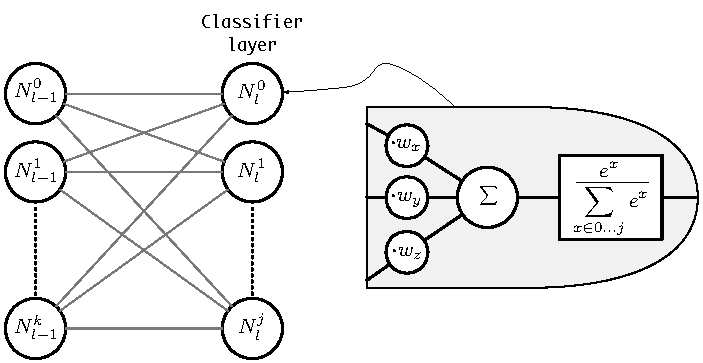
\includegraphics[angle=0, width=.65\textwidth]{classifierDiagram}}
    }
    \center\caption{Classifier layer}
    \label{fig:classifier layer}
  \end{minipage}
  \bigskip
  \vspace{0.5cm}
  \begin{minipage}{1\textwidth}
    \centering
    \centerline{
    \mbox{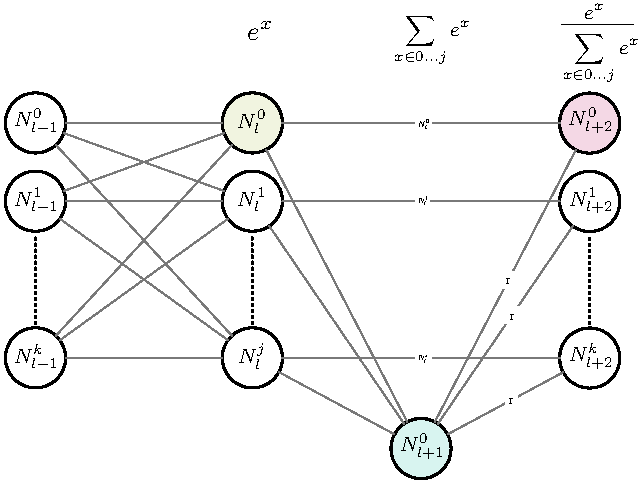
\includegraphics[angle=0, width=.55\textwidth]{classifierVirtualLayers}}
    }
    \caption{Classifier additional implementation layers}
    \label{fig:classifier additional layers}
  \end{minipage}
  %\captionof{figure}{Classifier}
  %\label{tab:Classifier}
\end{figure}

\begin{sidewaysfigure}[h]
  \centering
  \captionsetup{justification=centering}
  \captionsetup{width=0.9\textwidth}
  \begin{minipage}{1\textwidth}
    \centering
    \centerline{
    \mbox{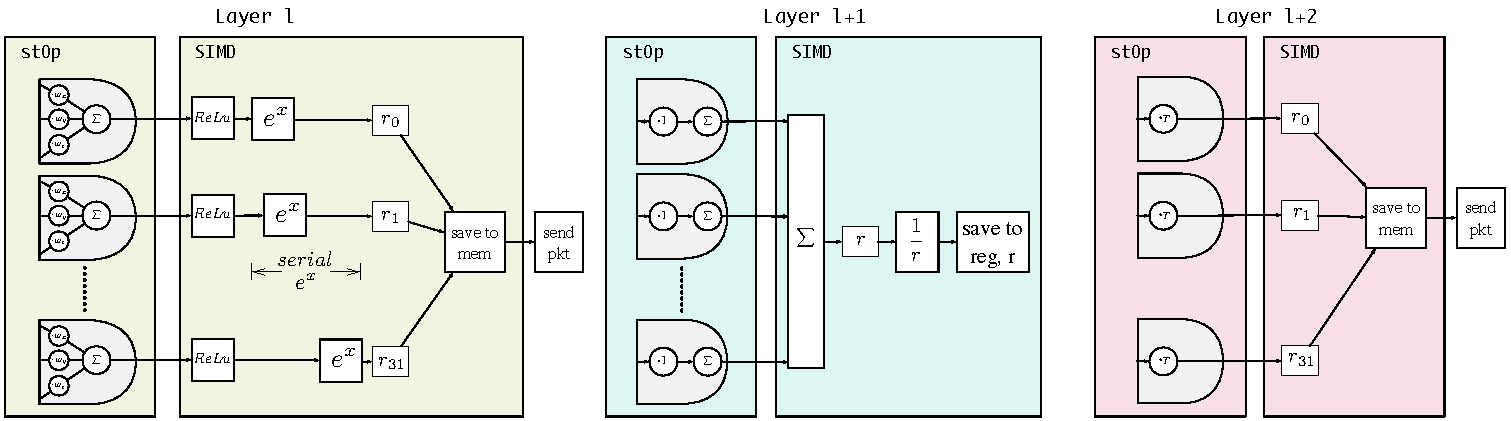
\includegraphics[angle=0, width=.95\textwidth]{classifierImplementation}}
    }
    \caption{Classifier layer stOp/SIMD implementation}
    \label{fig:classifier implementation}
  \end{minipage}
  \bigskip
  \vspace{5mm}
  \begin{minipage}{1\textwidth}
    \centering
    \centerline{
    \mbox{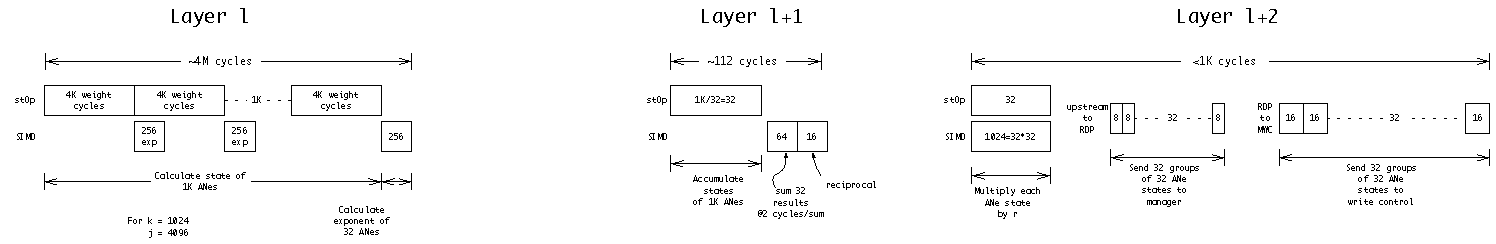
\includegraphics[angle=0, width=.95\textwidth]{classifierSequenceTiming}}
    }
    \center\caption{Classifier layer stOp/SIMD sequence timing}
    \label{fig:classifier implementation sequence timing}
  \end{minipage}
  %\captionof{table}{Classifier implementation}
  %\label{tab:Classifier implementation}
\end{sidewaysfigure}



\restoregeometry

%%---------------------------------------------------------------------------%%
%\ensureoddstart
\backmatter


\end{document}
